
%%%%%%%%%%%%%%%%%%%%%%%%%%%%%%%%%%%%%%%%%%%%%%%%%%%%%%%%%%%%%%%%%%%%%%%%%%%%
% AGUJournalTemplate.tex: this template file is for articles formatted with LaTeX
%
% This file includes commands and instructions
% given in the order necessary to produce a final output that will
% satisfy AGU requirements, including customized APA reference formatting.
%
% You may copy this file and give it your
% article name, and enter your text.
%
%
% Step 1: Set the \documentclass
%
%

%% To submit your paper:
\documentclass[draft]{agujournal2019}
\usepackage[utf8]{inputenc}
\usepackage{url} %this package should fix any errors with URLs in refs.
\usepackage{lineno}
\usepackage[finalnew]{trackchanges} %for better track changes. finalnew option will compile document with changes incorporated.
\usepackage{soul}
\usepackage{amsmath}
\linenumbers

\definecolor{psign}{rgb}{0.9  ,0.1,0.1}
\definecolor{pregime}{rgb}{0.9,0.5,0.0}
\definecolor{pregimet}{rgb}{0.6,0.2,0.2}
\definecolor{pexpo}{rgb}{0.1,0.4,0.7}

\newcommand{\op}{\operatorname}

\newcommand*\patchAmsMathEnvironmentForLineno[1]{%
  \expandafter\let\csname old#1\expandafter\endcsname\csname #1\endcsname
  \expandafter\let\csname oldend#1\expandafter\endcsname\csname end#1\endcsname
  \renewenvironment{#1}%
     {\linenomath\csname old#1\endcsname}%
     {\csname oldend#1\endcsname\endlinenomath}}%
\newcommand*\patchBothAmsMathEnvironmentsForLineno[1]{%
  \patchAmsMathEnvironmentForLineno{#1}%
  \patchAmsMathEnvironmentForLineno{#1*}}%
\AtBeginDocument{%
\patchBothAmsMathEnvironmentsForLineno{equation}%
\patchBothAmsMathEnvironmentsForLineno{align}%
\patchBothAmsMathEnvironmentsForLineno{flalign}%
\patchBothAmsMathEnvironmentsForLineno{alignat}%
\patchBothAmsMathEnvironmentsForLineno{gather}%
\patchBothAmsMathEnvironmentsForLineno{multline}%
}

%%%%%%%
% As of 2018 we recommend use of the TrackChanges package to mark revisions.
% The trackchanges package adds five new LaTeX commands:
%
%  \note[editor]{The note}
%  \annote[editor]{Text to annotate}{The note}
%  \add[editor]{Text to add}
%  \remove[editor]{Text to remove}
%  \change[editor]{Text to remove}{Text to add}
%
% complete documentation is here: http://trackchanges.sourceforge.net/
%%%%%%%

% \draftfalse

%% Enter journal name below.
%% Choose from this list of Journals:
%
% JGR: Atmospheres
% JGR: Biogeosciences
% JGR: Earth Surface
% JGR: Oceans
% JGR: Planets
% JGR: Solid Earth
% JGR: Space Physics
% Global Biogeochemical Cycles
% Geophysical Research Letters
% Paleoceanography and Paleoclimatology
% Radio Science
% Reviews of Geophysics
% Tectonics
% Space Weather
% Water Resources Research
% Geochemistry, Geophysics, Geosystems
% Journal of Advances in Modeling Earth Systems (JAMES)
% Earth's Future
% Earth and Space Science
% Geohealth
%
% ie, \journalname{Water Resources Research}

\journalname{Journal of Advances in Modeling Earth Systems}


\begin{document}

%% ------------------------------------------------------------------------ %%
%  Title
%
% (A title should be specific, informative, and brief. Use
% abbreviations only if they are defined in the abstract. Titles that
% start with general keywords then specific terms are optimized in
% searches)
%
%% ------------------------------------------------------------------------ %%

% Example: \title{This is a test title}

\title{\remove{Weather and climates in 16-bit arithmetics: }Number formats, error mitigation and scope \add{for 16-bit arithmetics in weather and climate modelling analysed with a shallow water model}}

%% ------------------------------------------------------------------------ %%
%
%  AUTHORS AND AFFILIATIONS
%
%% ------------------------------------------------------------------------ %%

% Authors are individuals who have significantly contributed to the
% research and preparation of the article. Group authors are allowed, if
% each author in the group is separately identified in an appendix.)

% List authors by first name or initial followed by last name and
% separated by commas. Use \affil{} to number affiliations, and
% \thanks{} for author notes.
% Additional author notes should be indicated with \thanks{} (for
% example, for current addresses).

% Example: \authors{A. B. Author\affil{1}\thanks{Current address, Antartica}, B. C. Author\affil{2,3}, and D. E.
% Author\affil{3,4}\thanks{Also funded by Monsanto.}}

\authors{M. Kl\"{o}wer\affil{1}, P. D. D\"{u}ben\affil{2}, and T. N. Palmer\affil{1}}


% \affiliation{1}{First Affiliation}
% \affiliation{2}{Second Affiliation}
% \affiliation{3}{Third Affiliation}
% \affiliation{4}{Fourth Affiliation}

\affiliation{1}{Atmospheric, Oceanic and Planetary Physics, University of Oxford, Oxford, UK}
\affiliation{2}{European Centre for Medium-Range Weather Forecasts, Reading, UK}
%(repeat as many times as is necessary)

%% Corresponding Author:
% Corresponding author mailing address and e-mail address:

% (include name and email addresses of the corresponding author.  More
% than one corresponding author is allowed in this LaTeX file and for
% publication; but only one corresponding author is allowed in our
% editorial system.)

% Example: \correspondingauthor{First and Last Name}{email@address.edu}

\correspondingauthor{M. Kl\"{o}wer}{milan.kloewer@physics.ox.ac.uk}

%% Keypoints, final entry on title page.

%  List up to three key points (at least one is required)
%  Key Points summarize the main points and conclusions of the article
%  Each must be 140 characters or fewer with no special characters or punctuation and must be complete sentences

% Example:
% \begin{keypoints}
% \item    List up to three key points (at least one is required)
% \item    Key Points summarize the main points and conclusions of the article
% \item    Each must be 140 characters or fewer with no special characters or punctuation and must be complete sentences
% \end{keypoints}

\begin{keypoints}
\item $\circ$ Posit numbers have smaller rounding errors compared to floating-point
 numbers in weather and climate applications, enabling reliable shallow water
 simulations computed entirely with 16-bit arithmetic.

\item $\circ$ Errors caused by 16-bit floating-point arithmetic are strongly
reduced with critical computations in 32 bit, which can be implemented on
present-day hardware.

\item $\circ$ 16 or even 8-bit communication between processors, preferably
encoded as posit numbers, introduces negligible errors, providing a perspective
for reduced data communication for weather and climate models.

\end{keypoints}

%% ------------------------------------------------------------------------ %%
%
%  ABSTRACT and PLAIN LANGUAGE SUMMARY
%
% A good Abstract will begin with a short description of the problem
% being addressed, briefly describe the new data or analyses, then
% briefly states the main conclusion(s) and how they are supported and
% uncertainties.

% The Plain Language Summary should be written for a broad audience,
% including journalists and the science-interested public, that will not have
% a background in your field.
%
% A Plain Language Summary is required in GRL, JGR: Planets, JGR: Biogeosciences,
% JGR: Oceans, G-Cubed, Reviews of Geophysics, and JAMES.
% see http://sharingscience.agu.org/creating-plain-language-summary/)
%
%% ------------------------------------------------------------------------ %%

%% \begin{abstract} starts the second page

\begin{abstract}
The need for high precision calculations with 64-bit or 32-bit floating-point
arithmetic for weather and climate models is questioned.
Lower precision numbers can accelerate simulations and are increasingly supported
by modern computing hardware. This paper investigates the potential of 16-bit
arithmetic when applied within a shallow water model that serves as a medium
complexity weather or climate application. There are several 16-bit number
formats that can potentially be used (IEEE half precision, BFloat16, posits,
integer and fixed-point). It is evident that a simple change to 16-bit arithmetic
will not be possible for complex weather and climate applications as it will
degrade model results by intolerable rounding errors that cause a stalling of
model dynamics or model instabilities. However, if the posit number format is
used as an alternative to the standard floating-point numbers the model degradation
can be \add{significantly} reduced\remove{ to a tolerable minimum}. Furthermore, a number of mitigation methods,
such as rescaling, reordering and mixed-precision, are available to make model
simulations resilient against a precision reduction. If mitigation methods are applied,
16-bit floating-point arithmetic can be used successfully within the shallow water model.
The results show the potential of 16-bit formats for at least parts of complex weather
and climate models where rounding errors would be entirely masked by initial
condition, model or discretization error.

\end{abstract}

%% ------------------------------------------------------------------------ %%
%
%  TEXT
%
%% ------------------------------------------------------------------------ %%

\section*{Plain Language Summary}

64-bit floating-point numbers are the standard number format for scientific
computing in fluid dynamics, which allows for very precise calculations with
negligible rounding errors. The need for calculations at this precision level
has been questioned for weather and climate models, as errors are caused
primarily by insufficient observations or deficiencies of the models themselves.
Reducing numerical precision can accelerate simulations and low precision number
formats are increasingly supported by modern computers. This paper investigates
the potential of low numerical precision with numbers that only use 16 bit of
information, when applied within weather and climate applications. There are
several 16-bit number formats that can potentially be used, all of which have
considerably larger rounding errors than the standard 64-bit numbers. In this
paper, the different number formats are applied in a two-dimensional oceanic or
atmospheric circulation model. A simple change to 16-bits for all calculations
will not be possible as it will degrade simulation results. However, if mitigation
methods are applied, 16-bit calculations can be used successfully within the
applications of this paper. The results show the potential of 16-bit number
formats for at least parts of complex weather and climate models.

\section{Introduction}
\label{sec:intro}

Predictions of weather and climate remain very difficult despite the use of the
world's fastest supercomputers. Although the available computational resources
have vastly increased over the last decades, forecast errors remain and have
several origins \cite{Palmer2012,Palmer2015}. They can be categorized as
initial and boundary condition errors, model errors and discretisation errors.
For instance, uncertainties in the observational data and their
assimilation contribute to the errors in the initial conditions; discrepancies
between the mathematical model and the real world cause model errors; and the finite
spatial and temporal resolution result in discretisation errors. The forecast error
is in general a combination and respective contributions can be different for
different variables and forecast lead times. 64-bit double precision floating-point
numbers (Float64) are used as the default option for weather and climate models \add{since
the 1980s with the rise of 64-bit computing}. The Float64 format introduces\remove{ mostly
negligible} rounding errors \add{that are largely negligible} compared to the
other mentioned sources of error.

Faster calculations and communication on computing architectures can be achieved
with reduced precision floating-point numbers, with a trade-off between speed
and precision. Deep learning algorithms require only low numerical precision but
high computational performance. The recent boom of machine learning applications
increased the demand on hardware-accelerated reduced precision calculations,
such that hardware developments increasingly offer more flexibility on
low precision number formats. While 16-bit arithmetic was not available for use
on commodity supercomputing hardware in the past, today most hardware vendors
offer the use of 16-bit formats, such as 16-bit half precision floating-point
numbers (Float16), on the next generation of hardware.

Graphic processing units started to support Float16 for increased performance
\cite{Markidis2018}. Google's tensor processing units (TPU, \citeA{Jouppi2017,Jouppi2018})
support the 16-bit BFloat16 format, a truncated version of \add{32-bit single-precision
floats (}Float32\add{)}, as this format is sufficiently precise for many deep learning
applications \cite{Kalamkar2019,Burgess2019,Gupta2015}. The world's fastest
supercomputers have reached peak performances of 100 Petaflop/s ($10^{17}$
floating-point operations per second) with Float64 in the last years, but peak
performances with Float16 are already beyond the exascale milestone
($10^{18}$ flop/s, \citeA{Kurth2018}).

A gained speed from low precision calculations can free resources
to increase the complexity and therefore the forecast skill in weather and climate models.
The European Centre for Medium-Range Weather Forecasts reduces the runtime by
40\% but not the forecast skill in their forecast model when using almost entirely
\remove{32-bit single precision (}Float32\remove{)} instead of Float64 \cite{Vana2017}. MeteoSwiss
profited similarly with Float32 in their forecast model \cite{Rudisuhli2013}. For
the European ocean model NEMO a mix of 32-bit and 64-bit arithmetic is a promising
approach to keep accuracy-critical parts in high precision while increasing
performance in others \cite{TintoPrims2019}.

Software emulators for other number formats than Float32 and Float64 are often
used to investigate rounding errors caused by lower precision formats \cite{Dawson2017}.
Although emulators are considerably slower than hardware-accelerated formats,
they allow a scientific evaluation of the introduced errors without requiring
specialised hardware, such as FPGAs \cite{Russell2017}. Unfortunately, the
computational performance cannot be assessed with software emulators.

Reducing the precision raises questions of the real bitwise information content.
In simplistic chaotic models only a minority of bits contain real information
\cite{Jeffress2017}, providing an information theoretic argument for reduced
precision calculations. Recent research covers reduced precision in
floating-point arithmetic in parts of weather forecast models\add{,
such as the dynamical core} \cite{Duben2014,Thornes2017,Chantry2019,Hatfield2020};
\add{physical parameterisations} \cite{Saffin2020};
\add{the ocean model} \cite{TintoPrims2019}; \add{the land-surface model} \cite{Dawson2018};
\add{data assimilation} \cite{Hatfield2017,Hatfield2018}. \remove{, but other number formats
than floats have gained little attention.} \add{In contrast to those studies,
we will evaluate various 16-bit arithmetics, as other formats than floats have
gained little attention, discuss options for reduced precision approaches and present
ways to mitigate rounding errors.}

Although floating-point numbers are the dominating number format in scientific
computing, alternatives have been proposed \cite{Gustafson2017a,Johnson2020}.
Posit\texttrademark ~numbers claim to provide more effective precision in algorithms
of machine learning and linear algebra \cite{Gustafson2017,Langroudi2019}, compared
to floats at the same word length. Posits were initially tested in simplistic
weather and climate simulations \cite{Klower2019a} -- research that is extended
here, providing a more thorough investigation of various 16-bit number formats.

Is 16-bit arithmetic useful within weather and climate models? Which 16-bit
formats are most promising, and can model simulations be made resilient
against a reduction in precision to 16 bits? These questions are covered in
this study. We apply several types of 16-bit arithmetic and test their impact
on the simulated dynamics in a shallow water model that serves as a medium-complexity
weather and climate application.

The study is structured as follows: Section \ref{sec:formats} outlines the
different number formats, the concept of decimal precision, and mitigation
methods to increase a model's tolerance for lower precision and a limited dynamic
range with 16-bit formats. Section \ref{sec:swm} presents results
of various implementations of 16-bit arithmetic in the shallow water model.
Section \ref{sec:discuss} discusses the results and provides the conclusions.

\section{16-bit number formats and mitigation methods}
\label{sec:formats}

This section discusses different types of 16-bit arithmetic, and similarities
and differences between them. Mitigation methods that allow for the use of
16-bit arithmetic within weather and climate applications are introduced.

\subsection{16-bit number formats}

\subsubsection{The integer and fixed point number format}
\label{sec:integer}

The simplest way to represent a real number in bits is the integer format.
An $n$-bit signed integer starts with a sign bit followed by a sequence of integer
bits, that are decoded as a sum of powers of 2 with exponents $0,1,...,n-2$.
The largest representable number $maxpos$ for a signed integer format is $2^{n-1}-1$.
Fixed-point numbers extend the integer format by adding $n_f$ fraction bits to
decode an additional sum of powers of 2 with negative exponents $-1,-2,...,-n_f$.
Every additional fraction bit reduces the number of integer bits. For example,
Q6.10 is the 16-bit fixed-point format with 6 signed integer bits and 10 fraction bits.

The arithmetic of fixed-point numbers is very similar to integers. The range of
representable numbers with integer arithmetic can therefore be
changed with fixed-point numbers, providing some flexibility for integer arithmetics
\cite{Russell2017}. However, the width of the dynamic range, $\log_{10}(maxpos/minpos)$,
is always limited and less than five orders of magnitude for any 16-bit integer
or fixed-point format -- too small for most applications. We will therefore focus
on the discussion of the other number formats in the rest of the study.

\subsubsection{The floating-point number format}
\label{sec:floats}

The IEEE standard on floating-point arithmetic defines how floats encode a real
number $x$ in terms of a sign, and several exponent and significant bits
\begin{equation}
x = (-1)^{sign~bit} \cdot 2^{e-bias} \cdot (1+f).
\label{eq:float}
\end{equation}
The exponent bits $e$ are interpreted as unsigned integers, such that $e-bias$
converts them effectively to signed integers. The fraction (or significant) bits
$f_i$ are defined as before, such that the significand $(1+f)$ is in the bounds
$[1,2)$. An 8-bit float encodes a real number with a sign bit (red), $n_e = 3$
exponent bits (blue) and $n_f=4$ fraction bits (black) as illustrated in the
following example
\begin{equation}
3.14 \approx {\color{psign}0}{\color{pexpo}100}1001_{\op{Float8}} =
(-1)^{\color{psign}0} \cdot 2^{{\color{pexpo}4}-bias} \cdot (1+2^{-1}+2^{-4}) =
3.125
\label{eq:posit_pos}
\end{equation}
with $bias=2^{n_e-1} - 1 = 3$. Exceptions to Eq. \ref{eq:float} occur for
subnormal numbers, infinity (Inf) and Not-a-Number (NaN) when all exponent bits
are either zero (subnormals) or one (Inf when f=0, or NaN else). 16-bit half-precision
floating point numbers (Float16) have 5 exponent bits and 10 significant bits.
A truncated version of the Float32 format (8 exponent bits, 23 significant bits)
is BFloat16 with 8 exponent bits and 7 significant bits. A format with more exponent
bits has a wider dynamic range of representable numbers but lower precision, as
fewer bits are available for the significand. All floating-point formats have a
fixed number of bits in the significand, consequently, they have a constant
number of significant digits throughout their range of representable numbers
(subnormals excluded).

\subsubsection{The posit number format}
\label{sec:posit_methods}

Posit numbers arise from a projection of the real axis onto a circle (Fig. \ref{fig:circle}),
with only one bit pattern for zero and one for Not-a-Real (NaR, also called \emph{complex infinity}),
which serves as a replacement for Not-a-Number (NaN) as well as positive and negative infinity.
The circle is split into \emph{regimes}, determined by a constant $useed$, which
always marks the north-west on the posit circle (Fig. \ref{fig:circle}b). Regimes
are defined by $useed^{\pm1}$, $useed^{\pm2}$, $useed^{\pm3}$, etc. which set a
wide dynamic range of representable numbers. To encode these regimes into bits,
posit numbers use regime bits which extend the standard on floating-point arithmetic.
Regime bits are a sequence of identical bits after the sign bit, terminated by an
opposite bit. As the number of regime bits is not fixed but flexible, the significand
increases in length for numbers towards $\pm1$, when fewer regime bits are needed.
Consequently, a higher precision around one can be achieved with posits, which
is traded against a gradually lower precision for very large or very small numbers.

A positive posit number $p$ is decoded as \cite{Gustafson2017,Gustafson2017a,Chen2018,Klower2019a}
\begin{equation}
p = (-1)^{sign~bit} \cdot useed^k \cdot 2^e \cdot (1+f).
\label{eq:posit}
\end{equation}
$k$ is the number of regime bits. $e$ is the unsigned integer encoded by the
exponent bits and $f$ is the fraction which is represented in the fraction
(or significant) bits. The base of the regime bits $useed = 2^{2^{e_s}}$ is
determined by the number of exponent bits $e_s$. More exponent bits $e_s=1,2,3,...$
increase $useed = 4,16,256,...$ and therefore widen the dynamic range of representable
numbers but reduce the precision around $\pm1$. The exponent bits themselves fill
gaps of powers of 2 spanned by $useed$ and so do not affect
the dynamic range directly by changing the value of $2^e$ in Eq. \ref{eq:posit}.
Consequently, every posit number, except for zero and NaR, can be written as
$p = \pm 2^i \cdot (1+f)$ for a given integer $i$. In the following,
a posit number format with $n$ bits including $e_s$ exponent bits
is denoted as Posit($n$,$e_s$).

We provide an example in the Posit(8,1)-system (i.e. $useed = 4$), which encodes
the number \change{14}{$\pi$} as follows
\begin{equation}
{\color{psign}0}{\color{pregime}1}{\color{pregimet}0}{\color{pexpo}1}1001_{\op{Posit}(8,1)}
= (-1)^{\color{psign}0} \cdot 4^{\color{pregime}0} \cdot 2^{\color{pexpo}1}
\cdot (1+2^{-1}+2^{-4}) = 3.125 \approx \pi.
\label{eq:posit_pos}
\end{equation}
The sign bit is red, regime bits orange, the terminating regime bit brown, the
exponent bit blue and the fraction bits are black. The $k$-value
\change{follows}{is derived} from the number of regime bits $n_r$\change{.}{, depending on whether
those are 0 or 1:} \change{For regime bits being 0 $k=-n_r$, for regime bits being 1 $k=n_r-1$,
in this example $k=0$.}{$k=-n_r$ if the regime bits are 0, but $k=n_r-1$ if the
regime bits are 1. In the example of Eq. 4, $k=1$ for 2 regime bits
of value 1.} The exponent bits are interpreted as unsigned integer and the fraction
bits follow the IEEE floating-point standard for significant bits.

\begin{figure}[htbp]
\center
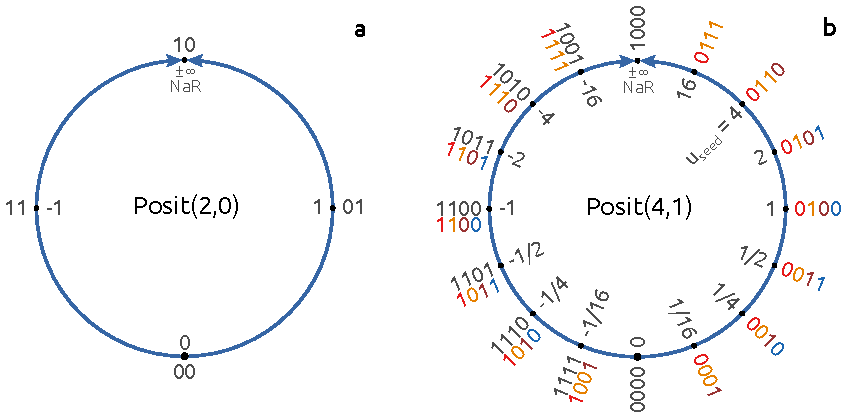
\includegraphics[width=1\textwidth]{circles.pdf}
\caption{Two posit number formats obtained by projecting the real axis onto a circle.
(a) 2-bit Posit(2,0) and (b) 4-bit Posit(4,1). The bit patterns are marked on the
outside and the respective values on the inside of each circle. Bit patterns of
negative numbers (black) have to be converted to their two's complement (colours)
first (see text). At the top of every circle is complex infinity ($\pm \infty$)
or NaR (Not-a-Real). After \citeA{Gustafson2017a}.}
\label{fig:circle}
\end{figure}

In order to use posits on a conventional processor we developed for the Julia
programming language \cite{Bezanson2017} the posit emulator \emph{SoftPosit.jl}
\cite{Klower2019} as bindings for the C-based library SoftPosit \cite{Leong2020}.
A standardized posit processor is not yet available, but current research focuses
on hardware implementations \cite{Zhang2020,vanDam2019,Chen2018,Chaurasiya2018,Glaser2017}.

\subsection{\change{The concept of d}{D}ecimal precision and summary of number formats}
\label{sec:decprec}

Most arithmetic operations include rounding of an exact result $x_\text{exact}$
to a representable number $x_\text{repr}$. Based on the decimal rounding error
$\vert \log_{10}( \tfrac{x_\text{repr}}{x_\text{exact}} ) \vert$ the decimal precision
is defined as \cite{Gustafson2017, Klower2019a}
\begin{equation}
\op{decimal} \op{precision} = -\log_{10} \vert \log_{10}( \frac{x_\text{repr}}{x_\text{exact}} ) \vert.
\end{equation}
The decimal precision measures the number of correct decimal places after rounding.
The decimal precision goes to infinity when the exact result approaches a
representable number. Rounding an exact result half-way between two representable
numbers maximises the decimal error and minimises the decimal precision.
This minimum is the \emph{worst-case} decimal precision, which measures the number
of decimal places that are at least correct after round-to-nearest. In the following
we will refer to the worst-case decimal precision simply as decimal precision.
The machine epsilon $\epsilon$, a relative rounding error in floating-point arithmetic,
is commonly used to measure the precision of number formats. It is defined as the
distance $\delta$ between 1 and the next largest representable number, and can be
given in terms of decimal precision as $\epsilon = -\log_{10} ( \log_{10}( 1 + \tfrac{\delta}{2} ))$.

\begin{figure}[htbp]
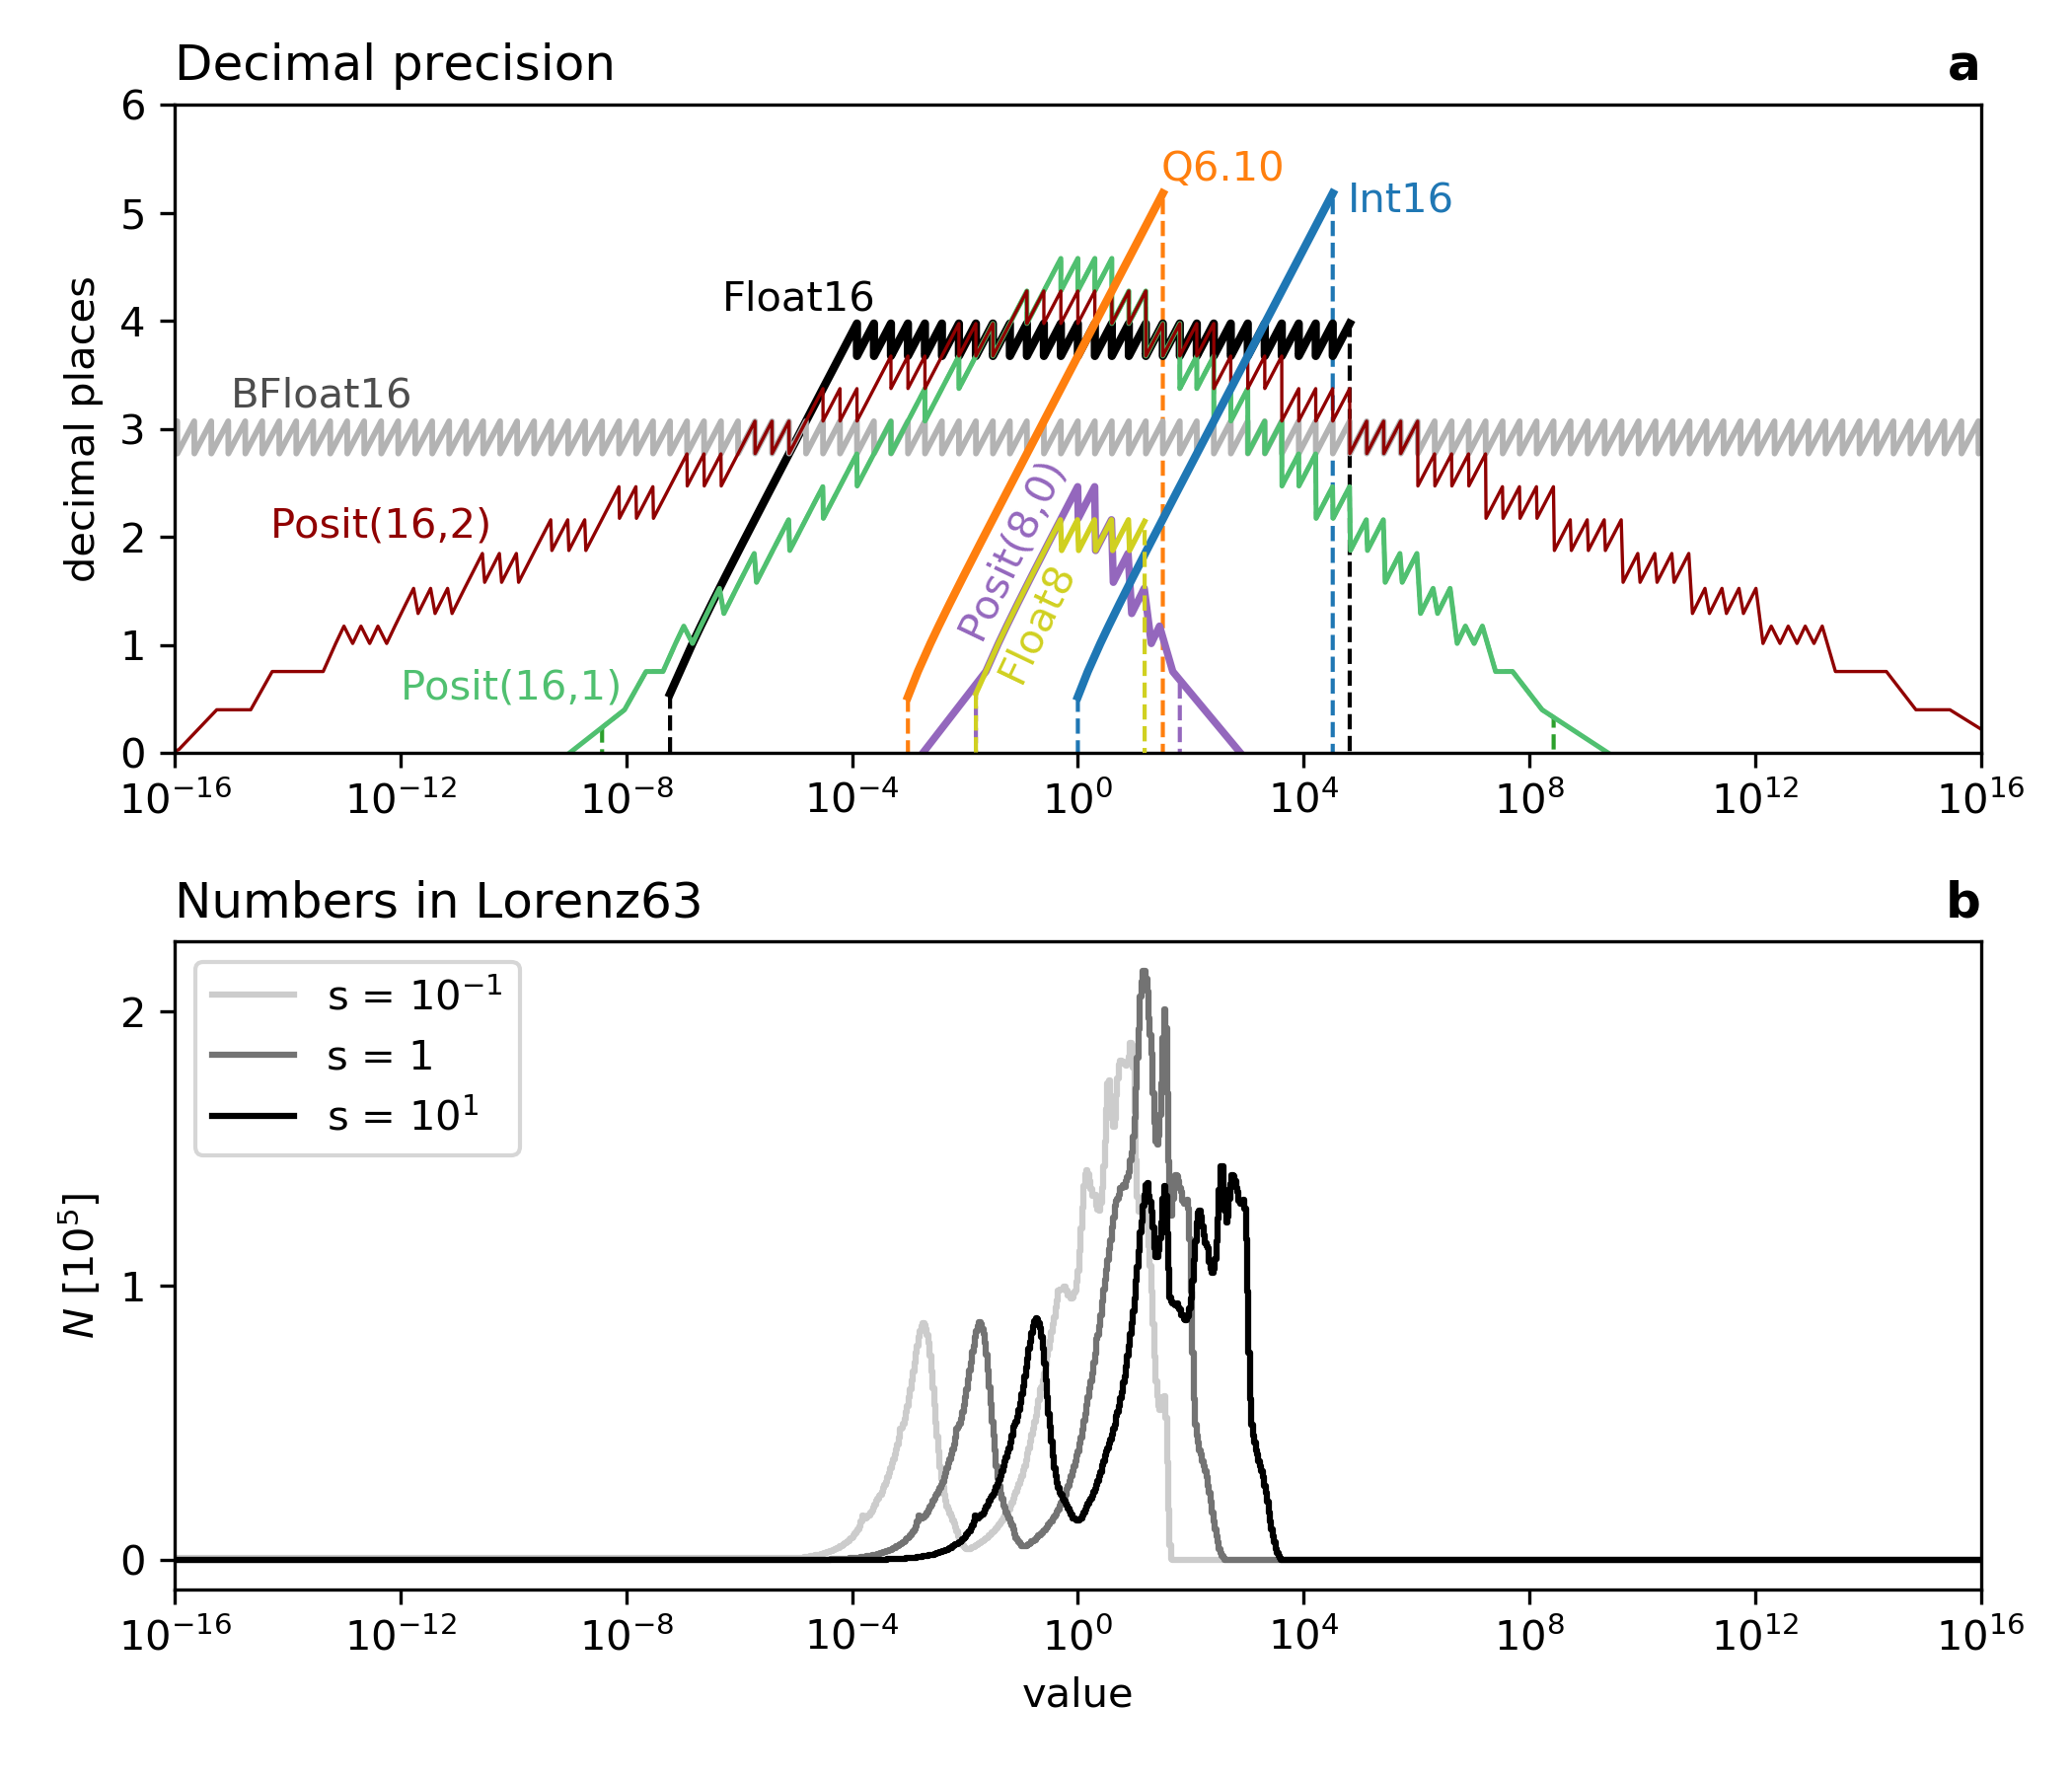
\includegraphics[width=1\textwidth]{decimal_precision.png}
\caption{(a) Decimal precision for various number formats. Dashed vertical lines
indicate for each format the range from $minpos$ to $maxpos$ of representable numbers.
Float64, Float32 and Posit32 are beyond the axes limits. (b) Histogram of results
of the absolute values of all arithmetic operations in Lorenz system rescaled by $s$.}
\label{fig:dec_prec}
\end{figure}

The decimal precision for various 16 and 8-bit floats and posits, 16-bit integers
and the fixed-point format Q6.10 (6 integer bits, 10 fraction bits) is presented
in Fig. \ref{fig:dec_prec}a. Floats have an exponent that is evenly spaced in
logarithmic-space, which results in a nearly constant decimal precision. The deviations
from a constant decimal precision, which can be seen as regular spikes in Fig. \ref{fig:dec_prec}a,
are due to a linearly-spaced significand. The decimal precision for floats decreases
for the subnormal numbers towards the smallest representable number $minpos$.
Posits have an increased decimal precision around 1 and a wide dynamic range,
due to the tapered precision towards $minpos$ and the largest representable number
$maxpos$. The decimal precision for posits is above zero outside the dynamic range
as posits have a no overflow/no underflow-rounding mode. Integers are linearly-spaced,
consequently their precision increases towards $maxpos$ for 16-bit signed integers.
The decimal precision of fixed-point numbers has an identical shape, but is shifted
towards smaller numbers by a factor of $\tfrac{1}{2}$ for each additional fraction bit.
Consequently, many arithmetic calculations should be placed close to $maxpos$, but
the small range of high precision is restrictive for many applications. No convincing results
with integer or fixed-point arithmetic were achieved in this study, especially as
the limited dynamic range of less than five orders of magnitude imposes a very difficult
constrain to avoid under- or overflows.

\begin{table}[htbp]
\center
\begin{tabular}{l | r | r | l | l | r | r}
Format & bits & exp bits & $minpos$ & $maxpos$ & $\epsilon$ &  \% NaR \\
\hline
Float64    & 64 & 11 & $5.0 \cdot 10^{-324}$ & $1.8 \cdot 10^{308}$  & 16.3 & 0.0 \\
Float32    & 32 & 8 & $1.0 \cdot 10^{-45}$ & $3.4 \cdot 10^{38}$ & 7.6 & 0.4 \\
Float16    & 16 & 5 & $6.0 \cdot 10^{-8}$ & 65504 & 3.7 & 3.1 \\
BFloat16    & 16 & 8 & $ 9.2 \cdot 10^{-41}$ & $3.4 \cdot 10^{38}$ & 2.8 & 0.4  \\
Float8 & 8 & 3 & $1.5 \cdot 10^{-2}$ & 15.5 & 1.9 &12.5\\
\hline
Posit32    & 32 & 2 &  $7.5 \cdot 10^{-37}$ & $7.5 \cdot 10^{37}$ & 8.8 & 0.0 \\
Posit(16,1) & 16 & 1 & $3.7 \cdot 10^{-9}$ & $3.7 \cdot 10^{9}$ & 4.3 & 0.0\\
Posit(16,2) & 16 & 2 & $1.4 \cdot 10^{-17}$ & $1.4 \cdot 10^{17}$ & 4.0 & 0.0\\
Posit(8,0) & 8 & 0 & $1.5 \cdot 10^{-2}$ & 64 & 2.2 & 0.4  \\
\hline
Int16 & 16 & 0 & 1 & 32767 & 0.8 & 0\\
Q6.10 & 16 & 0 & $9.8 \cdot 10^{-4}$ & 32.0 & 3.7 & 0
\end{tabular}
\vspace{10pt}
\caption{Characteristics of various number formats. $minpos$ is the smallest
representable positive number, $maxpos$ the largest. The machine error $\epsilon$
is here given as decimal precision (i.e. correct decimal places after rounding).
\% NaR denotes the percentage of bit patterns that represent not a number (NaN),
infinity or not a real (NaR).}
\label{tab:formats}
\end{table}

Characteristics of various formats are summarised in Table \ref{tab:formats}.
Float64 has more than $10^{15}$ bit patterns reserved for NaN, but these only
make up $< 0.05\%$ of all available bit patterns. However, the percentage of
redundant bit patterns for NaN increases for floats with fewer exponent bits
and poses a noticeable issue for Float16 and Float8. Every posit number format
has only one bit pattern reserved for NaR, such that this issue is negligible for
posits.

\subsection{\change{M}{Approaches and m}itigation measures to allow for the use of 16-bit \change{arithmetic}{number formats} in
weather and climate applications}

\subsubsection{Mixed precision arithmetic}

In many models, it will not be possible (or useful) to use 16-bit arithmetic
throughout the entire model. Some model components will be more sensitive to a
reduction in precision when compared to others and it often makes sense to reduce
precision only in those components where results are not deteriorated, while
keeping precision high in precision-sensitive components. This approach is
called \emph{mixed-precision} and is already used for the reduction to single
precision in ocean and atmosphere models \cite{Vana2017,TintoPrims2019}.

\subsubsection{Algorithmic changes: Rescaling, reordering and precomputations}

Equations can be \emph{rescaled} via multiplication with a constant rescaling
factor $s$ to shift the dynamic range occurring in an algorithm towards larger
numbers (for $s > 1$) or towards smaller numbers ($s < 1$).
Rescaling can be used to adjust the number range to the decimal precision of the
number formats. If nonlinear terms are considered, this multiplicative rescaling
is ineffective, as the rescaling factor $s$ appears inside the non-linear terms.
The nonlinear terms are therefore effectively invariant under multiplicative
rescaling and only the linear terms are scaled by $s$.
Fig. \ref{fig:dec_prec} includes histograms of numbers occurring in the rescaled
Lorenz system \cite{Lorenz1963,Kwasniok2014,Jeffress2017,Tantet2018} as an example
from \citeA{Klower2019a}. For posit arithmetic it is preferable to use
$s=\tfrac{1}{10}$ in the Lorenz system to scale the prognostic variables
to match the range of highest decimal precision around $\pm1$, which increases the
complexity of the Lorenz attractor and decreases the average rounding error.

Furthermore, it is sometimes possible to avoid intermediate arithmetic results,
which may be outside the dynamic range of a number format, by changing the order
in which multiplications and divisions are executed. In general, it is preferable
to combine such operations to a single multiplication with a constant which can
be precomputed. Although this will have a negligible effect on the rounding error
for floating-point arithmetic due to the approximately constant decimal precision
throughout the range of numbers (subnormals excluded), it reduces the risk of
over- or underflow. Re-ordering the shallow water equations is discussed in
section \ref{sec:swm_rescale}.

\subsubsection{Reduced precision communication}

Complex weather and climate models rely on parallelisation to distribute the
computational cost of simulations efficiently among the processing units in a
large cluster or supercomputer. Parallel execution typically requires domain
decomposition, where the spatial domain is split into many subdomains to be
calculated separately on individual processing units. Domain decomposition
requires communication of the boundary values of a subdomain with the
neighbouring subdomains. If 16-bit arithmetic cannot be used within the
entire model, it may still be possible to reduce precision in the communication
between processors.

Not all weather and climate models would benefit from a reduced precision
communication as the acceleration potential depends on many factors specific
to a model and the used hardware, e.g. number of nodes in a cluster and how
shared and distributed memory is managed. It will also be important
whether communication is latency or volume bound. Latency bound communication is
bound by the time a package of information requires to travel between processors.
In contrast, volume bound communication is limited by the bandwidth that is
available for communication. Only the latter will benefit from a reduction in data
volume, which can be achieved with reducing precision.

However, if communication volume is an identified bottleneck in a given application,
which is often the case in weather and climate models, reliable model simulations
might be possible with 16 or even 8-bit communication, allowing for a significant
reduction in computing time. In general, various lossy and lossless data compression
techniques can be used to reduce communication volume \cite{Fan2019}. \add{Lossless
communication allows for bit-reproducible results when compared to simulations that
do not use compressed communication. We therefore} restrict ourselves to lossy type
conversions\change{, which introduce likely a negligible overhead
due to encoding before and decoding after communication.}{ which introduce rounding
errors to the data that is sent around while the overhead due to encoding before
and decoding after communication remains small.}

\section{A shallow water model with 16-bit arithmetic}
\label{sec:swm}

In this section, the different number formats Float16, BFloat16, Posit(16,1) and
Posit(16,2) are evaluated when solving the shallow water equations. The shallow
water model used here is an updated version of the one used in \citeA{Klower2019a},
and most details described therein are also valid here. A vertical integration of
the Navier-Stokes equations yields the shallow water equations, that can be used
to understand many features of the general circulation of atmosphere and ocean as
well as some two-dimensional non-linear interactions on shorter length and time scales
\cite{Gill1982,Vallis2006}. The shallow water equations for the prognostic variables
velocity $\mathbf{u} = (u,v)$ and sea surface elevation $\eta$ are
\begin{subequations}
\begin{align}
\frac{\partial \mathbf{u}}{\partial t} &+ (\mathbf{u} \cdot \nabla) \mathbf{u} +
f\hat{\mathbf{z}} \times \mathbf{u} = -g\nabla \eta + \mathbf{D} + \mathbf{F} \\
\frac{\partial \eta}{\partial t} &+ \nabla \cdot (\mathbf{u}h) = 0.
\end{align}
\label{eq:swe}%
\end{subequations}
$\eta$ can be interpreted as pressure for the atmosphere \cite{Gill1982}.
The shallow water system is forced with a zonal wind stress $\mathbf{F}$.
The dissipation term $\mathbf{D}$ removes energy on large scales (bottom friction)
and on small scales (diffusion). The non-linear term $(\mathbf{u} \cdot \nabla) \mathbf{u}$
represents advection of momentum. The term $f\hat{\mathbf{z}} \times \mathbf{u}$
is the Coriolis force and $-g\nabla \eta$ is the pressure gradient force, with
$g$ being the gravitational acceleration. Eq. \ref{eq:swe}b is the shallow
water-variant of the continuity equation, ensuring conservation of mass.

The shallow water equations are solved in the $(x,y)$-plane over the zonally periodic
rectangular domain $L_x \times L_y$, of size $2000\op{km} \times 1000\op{km}$.
We associate $x$ with the zonal and $y$ with the meridional direction. The domain
is centred at 45N with the beta-plane approximation \cite{Vallis2006}. The boundary
conditions are periodic in zonal direction and no-slip at the northern and southern
boundary. The layer thickness is $h = \eta + H(x)$, with
\begin{equation}
H(x) = H_0 - H_1\exp\left(-H_\sigma^{-2}(x-\tfrac{L_x}{2})^2\right)
\end{equation}
being the undisturbed depth, representing a meridional mountain ridge at
$x=\tfrac{L_x}{2}$ spanning from the southern to the northern boundary.
The standard depth is $H_0 = 500\op{m}$. The ridge has a maximum height of
$H_1 = 50\op{m}$ and a characteristic width of $H_\sigma = 300\op{km}$, which
makes the zonal current barotropically unstable. The flow regime is therefore
governed both by eddy-mean flow as well as eddy-eddy interactions.

The time step $\Delta t = 282\op{s}$ is chosen to resolve surface gravity waves,
traveling at an estimated phase speed of $\sqrt{gH_0}$ with a CFL number close to
1 and gravitational acceleration $g=10\op{ms}^{-1}$. The wind stress
forcing $\mathbf{F} = (F_x,0)$ is constant in time, acts only on the zonal momentum
budget
\begin{equation}
Fx = \frac{F_0}{\rho h} \cos\left(\pi\left(y{L_y}^{-1} - 1\right)\right)^2
\end{equation}
and vanishes at the boundaries. The water density is $\rho = 1000\op{kg}\op{m}^{-3}$
and $F_0 = 0.12\op{Pa}$. The wind forcing acts as a continuous input of large-scale
kinetic energy that is balanced by the dissipation term.

The dissipation term $\mathbf{D}$ is the sum
\begin{equation}
\mathbf{D} = -\frac{c_D}{h}\| \mathbf{u} \| \mathbf{u} - \nu \nabla^4 \mathbf{u}
\label{eq:diss}
\end{equation}
of a quadratic bottom drag with dimensionless coefficient $c_D = 10^{-5}$ \cite{Arbic2008}
and a biharmonic diffusion with viscosity coefficient $\nu \approx 1.33\times10^{11} \op{m}^4\op{s}^{-1}$ \cite{Griffies2000}.

The shallow water equations are discretized using 2nd order centred finite differences
on an Arakawa C-grid \cite{Arakawa1977} and the fourth-order Runge-Kutta method \cite{Butcher2016}
is used for time integration of the pressure, Coriolis and advective terms, whereas a
semi-implicit method is used for the dissipative terms $\mathbf{D}$. We present results
of simulations with three different levels of resolution: high resolution simulations
with a grid spacing of $\Delta = 5\operatorname{km}$ (400x200 grid points), medium
resolution simulations with a grid-spacing of $\Delta = 20\operatorname{km}$
(100x50 grid points) and low resolution with a grid-spacing of $\Delta = 40\operatorname{km}$
(50x25 grid points). The advection terms are discretized using an energy and
enstrophy conserving scheme \cite{Arakawa1990}.

The shallow water equations are extended with an advection equation for tracers.
Temperature and humidity or salinity are examples of tracers in the atmosphere
and the ocean. For simplicity, we regard them as passive here, such that they do not
influence the flow. The advection of a passive tracer $q$ given a velocity $\mathbf{u}$
is governed by
\begin{equation}
\frac{\partial q}{\partial t} + \mathbf{u} \cdot \nabla q = 0.
\label{eq:adv}
\end{equation}
A semi-Lagrangian advection scheme \cite{Smolarkiewicz1992} is used to discretise
Eq. \ref{eq:adv}. In this discretization, the tracer concentration for a given grid cell
(i.e. the arrival point) is calculated from the concentration at a departure point
at the previous time step. The departure point is determined by back-tracing the
velocities from the arrival point. Departure points in general
do not coincide with grid nodes, such that an interpolation from the surrounding grid
points is required to find the concentration at the departure point, which is then
defined to be the concentration at the arrival point.

\subsection{Rescaling the shallow water equations}
\label{sec:swm_rescale}

The dynamic range of representable numbers with 16-bit arithmetic is for most
formats discussed here considerably smaller than with Float32 or 64
(Fig. \ref{fig:dec_prec}a and Table \ref{tab:formats}). It is therefore
important to rescale the calculations to limit the range of
arithmetic results to stay within the bounds of a given 16-bit format.

The prognostic variables in the shallow water equations are typically
$\mathcal{O}(1\op{ms}^{-1})$ for $\mathbf{u}$, $\mathcal{O}(1\op{m})$ for
$\eta$ and $\mathcal{O}(1)$ for $q$. Their physical units are therefore retained
in the discretised numerical model and we do not apply a rescaling of the shallow
water equations as a whole. However, the grid spacing $\Delta$ in units of meter
is large for geophysical flows. We therefore use dimensionless Nabla operators
$\tilde{\nabla} = \Delta\nabla$. The continuity equation Eq. \ref{eq:swe}b,
for example, reads then as
\begin{equation}
\eta^{n+1} = \eta^n + \tilde{\Delta t}\left( - \tilde{\nabla} \cdot (\mathbf{u}h)^n\right)
\label{eq:discr}
\end{equation}
for an explicit time stepping scheme. $\tilde{\Delta t}$ is the rescaled time
step, a Runge-Kutta coefficient times $\tfrac{\Delta t}{\Delta}$ to combine a
division by a large value for $\Delta$ and a subsequent multiplication with a
large value for $\Delta t$ into a single multiplication with $\tilde{\Delta t}$.
The other terms are rescaled accordingly ($\tilde{f} = f\Delta$;
$\tilde{\mathbf{F}} = \mathbf{F}\Delta$). As these terms remain constant, they
can be precomputed at higher precision during model initialisation.
The momentum equations are rescaled similarly.

Diffusion is an example of a discretization scheme that requires rescaling for
the arithmetic results to fit into the limited dynamic range. Biharmonic diffusion
\cite{Griffies2000} calculates a fourth-derivative in space,
which is often very small $\mathcal{O}(10^{-20})$ in geophysical applications,
due to the large physical dimensions, when using meters as a unit for length.
Contrarily, biharmonic viscosity coefficients are typically very large
$\mathcal{O}(10^{11})$.
We therefore rescale $\mathbf{D}$ accordingly
\begin{equation}
\tilde{\mathbf{D}} =-\frac{\tilde{c_D}}{h}\| \mathbf{u} \| \mathbf{u} -
\tilde{\nu}\tilde{\nabla}^4\mathbf{u}
\end{equation}
with $\tilde{c_D} = c_D\Delta = 0.2\op{m}$,  and $\tilde{\nu} = \nu\Delta^{-3}
\approx 0.16\op{ms}^{-1}$, which are precomputed. The term
$\tilde{\mathbf{D}}$ is computed instead of $\mathbf{D}$ and the scaling eventually
undone when multiplying with the rescaled time step $\tilde{\Delta t}$.

The semi-Lagrangian advection scheme is reformulateed for 16-bit arithmetics.
In the absence of sources and sinks, the Lagrangian point-of-view states that
the tracer concentration $q$ does not change following a flow trajectory.
The concentration $q$ at departure points $\mathbf{x}_d$ at time $t$ is therefore
the same as the concentration at time $t+\Delta t_{\op{adv}}$ at arrival points
$\mathbf{x}_a$, which are chosen to coincide with the grid points.
Based on the flow velocity at the arrival point, the departure point is derived.
To avoid large numbers for the coordinates (in our case $L_x = 2 \cdot 10^6$m),
non-dimensional departure points $\mathbf{\tilde{x}}_{d,rel}$ relative to the
arrival point are computed as
\begin{equation}
\mathbf{\tilde{x}}_{d,rel} = - \mathbf{u}(\mathbf{x}_a,t+\Delta t_{\op{adv}})
\left( \frac{\Delta t_{\op{adv}}}{\Delta} \right).
\label{eq:relcoord}
\end{equation}
A scaling with the grid-spacing inverse $\Delta^{-1}$ is applied such that all
terms are $\mathcal{O}(1)$ and therefore representable with 16-bit arithmetics.
In practice, when converting the relative departure point $\mathbf{\tilde{x}}_{d,rel}$
to an array index for the interpolation, the floor function is used in combination
with integer arithmetics. This essentially separates a computation with reals
into two parts. One that can be computed with integers without rounding errors,
and a calculation with reals, with a removed offset to reduce rounding errors.

\subsection{Shallow water simulations in 16-bit arithmetic}

\begin{figure}
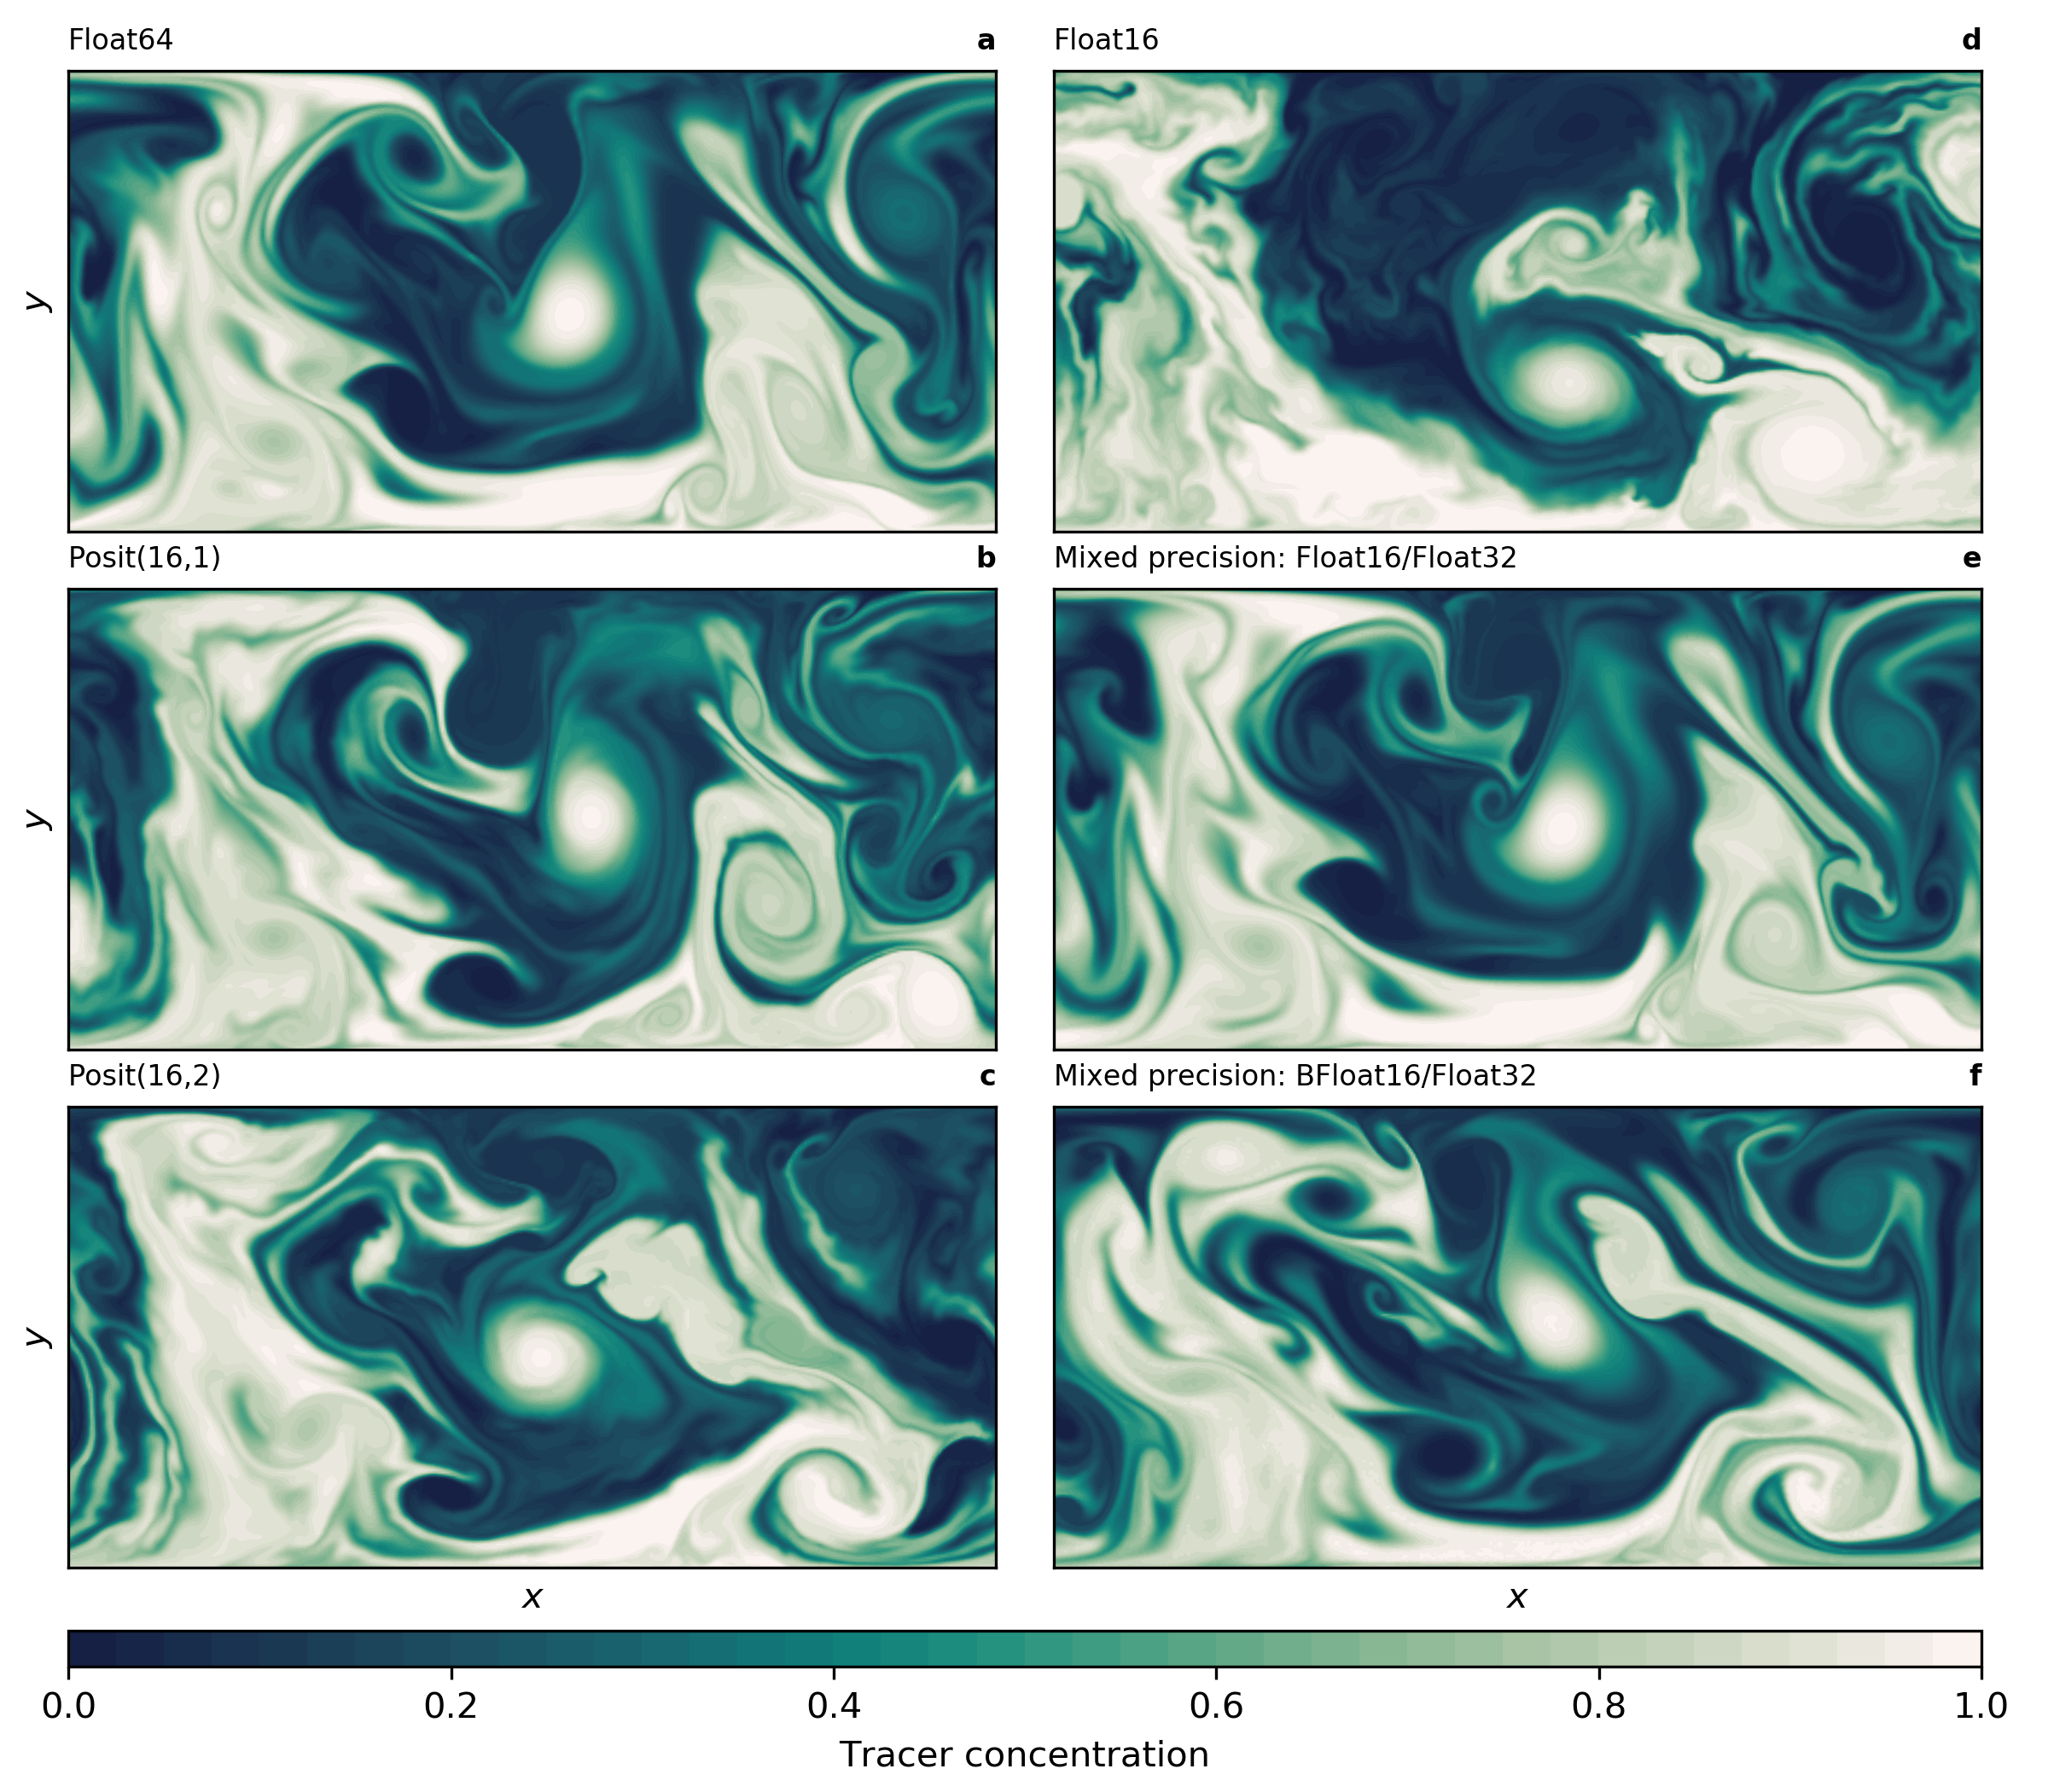
\includegraphics[width=1\textwidth]{snapshot.png}
\caption{Snapshot of tracer concentration simulated by the shallow water model
using different 16-bit number formats and the high-resolution configuration
($\Delta = 5$km). The mixed precision simulations presented in (e) and (f) are
using Float32 for the representation of prognostic variables only. The tracer
was injected uniformly in the lower half of the domain 50 simulation days before
the time step shown.}
\label{fig:snapshot}
\end{figure}

The shallow water model simulates vigorous turbulence interacting with a
zonal current (Fig. \ref{fig:snapshot}). Both float and posit arithmetic
present very similar fluid dynamics in comparison to the Float64 reference in
only 16 bit. A snapshot of tracer concentration many simulated days after
initialisation reveals turbulent mixing of the tracer that is well simulated
with posits. However, with Float16 the simulation deviates faster from the
reference than with Posit(16,1) and to a lesser degree with Posit(16,2),
presumably due to the small scale instabilities visible in the snapshot as
wavy filaments and fronts. These instabilities are clearly triggered by Float16
arithmetics, but to a lower degree also visible for posits. This provides some
visual evidence that accumulated rounding errors are reduced with posits, especially
Posit(16,1). BFloat16 arithmetic is not able to simulate the shallow water dynamics,
as tendencies are too small to be added to the prognostic variables. A stalling
of the simulated flow is observed. \add{The results with mixed precision,
Float16/Float32 and BFloat16/Float32, will be discussed in section 3.3.}

\begin{figure}
\includegraphics[width=1\textwidth]{rmse_eta_darker.pdf}
\caption{Forecast error of sea surface height $\eta$ measured as root mean square
error (RMSE) taking Float64 as reference. (a) Forecast error for various 16-bit
number formats and mixed 16/32-bit simulations for which the prognostic variables
are kept in Float32. (b) Forecast error for reduced precision communication in
8 or 16 bit with various number formats used for encoding, with Float64 used for
all calculations. The communication of boundary values occurs at every time step
for the prognostic variables. The RMSE is normalised by a mean forecast error at
very long lead times. Solid lines represent the median of 200 forecasts per number
format. The shaded areas of each model configuration denote the interquartile
range of the forecast experiments.}
\label{fig:rmse}
\end{figure}

Short-term forecasts at medium-resolution ($\Delta = 10$km) are performed to
analyse the differences between different 16-bit arithmetics. To quantify the error
growth caused by rounding errors with different arithmetics in a statistically
robust way, we create a number of forecasts with each member starting from one
of 200 randomly picked start dates from a 50-year long control simulation. The
forecast error in the shallow water model is computed as root mean square error
(RMSE) of sea surface height $\eta$ with respect to Float64 simulations. Other
variables yield similar results. Each forecast is performed several times from
identical initial conditions but with the various number formats. The error growth
caused by rounding errors is additionally compared to the error
introduced by discretisation. A low-resolution model configuration with
$\Delta = 20$km is used to quantify a realistic level of discretisation error.
The RMSE is normalised by the climatological mean forecast error at very long lead
times, which is the same for all model configurations. When the normalised RMSE
reaches 1 all information on the initial conditions is removed by the chaotic
evolution of the shallow water system.

The forecast error of Float16 is as large as the discretisation error and
clearly outperformed by 16-bit posit arithmetic (Fig. \ref{fig:rmse}a).
Both Posit(16,1) and Posit(16,2) yield a forecast error that is several times
smaller than Float16. The forecast error of 32-bit arithmetic is several orders
of magnitude smaller and is only after 200 days as large as the error for 16-bit
arithmetic at short lead times of about 10 days. Also at 32 bit, posits clearly
outperform floats.

\begin{figure}
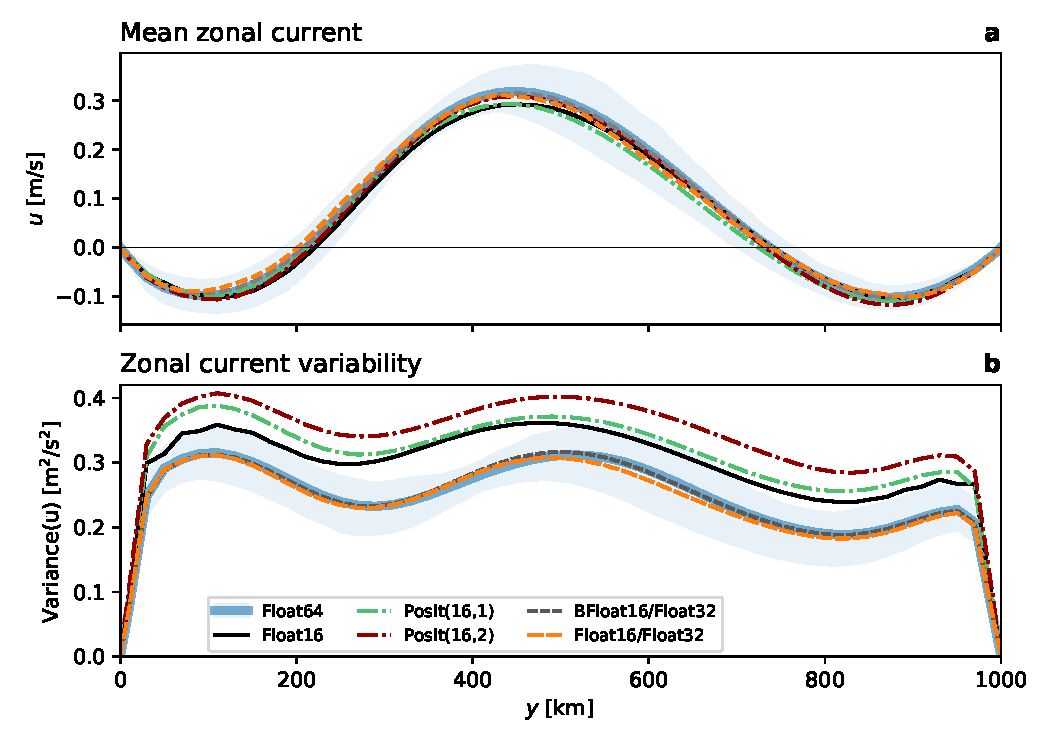
\includegraphics[width=1\textwidth]{meanvar_u.pdf}
\caption{Climatology and variability of the zonal current in the medium-resolution
simulations. (a) Zonally-averaged zonal current $u$ as a function of the meridional
coordinate $y$. (b) Zonal variance of the zonal current as a function of $y$.
\add{The dashed lines for BFloat16/Float32 and Float16/Float32 are almost identical.}
The shaded area denotes the interquartile temporal variability around the (a) mean and
(b) variance of reference simulation with Float64.}
\label{fig:mean}
\end{figure}

To investigate the effect of rounding errors on the climatological mean state of
the shallow water system, we zonally average the zonal velocity $u$. \add{This average
is based on 300-day long simulations starting from 200 different initial conditions,
which cover the various states in the long-term variability of the shallow water system.
However, the climatology from a single very long simulation has not been assessed.}

The mean state is an eastward flow of about 0.3~m/s, about 3 to 4 times weaker than
individual velocities throughout the domain (Fig. \ref{fig:mean}a), which is typical
for turbulent flows. A weak westward mean flow is found at the northern and
southern boundary. No 16-bit format was found to have a significant impact on
the mean state. The variability of the flow around its mean state is high
throughout the domain (Fig. \ref{fig:mean}b). The variability is significantly
increased by 10 -- 30\% with 16-bit arithmetic, especially with Posit(16,2).
This is probably caused by rounding errors that are triggering local
perturbations which increase variability.

\begin{figure}
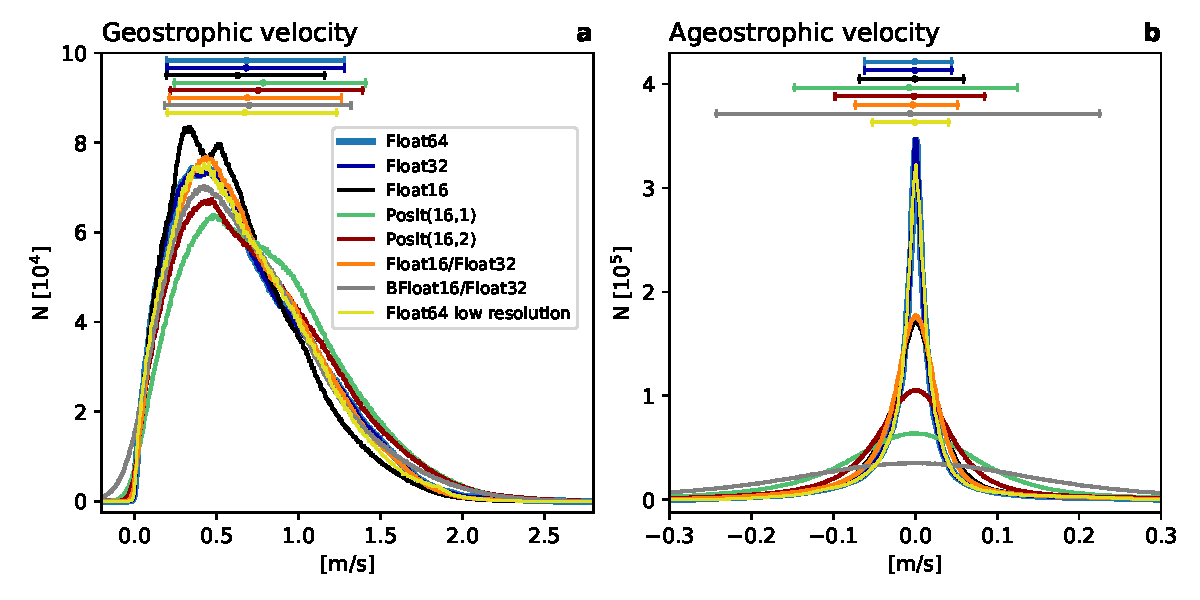
\includegraphics[width=1\textwidth]{ageostrophic.pdf}
\caption{Geostrophic balance as simulated with different number formats.
(a) Histograms of flow-parallel components of geostrophic velocity.
(b) as (a) but for the ageostrophic velocities. Horizontal bars denote the
mean, 10th and 90th-percentile in respective colours.}
\label{fig:geo}
\end{figure}

The turbulence in shallow water simulations is largely geostrophic, such that the
pressure gradient force opposes the Coriolis force. The resulting geostrophic
velocities $\mathbf{u}_g$ can be derived from the sea surface height $\eta$ as
\begin{subequations}
\begin{align}
\mathbf{u}_g &= \frac{g}{f}\hat{\mathbf{z}} \times \nabla \eta \\
\mathbf{u} &= \mathbf{u}_{g} + \mathbf{u}_{ag}
\end{align}
\label{eq:geo}%
\end{subequations}
and deviations from the actual flow $\mathbf{u}$ are the ageostrophic velocity
components $\mathbf{u}_{ag}$. We project both components on the actual velocities
to obtain the flow-parallel components $\tilde{u}_{g}$ and $\tilde{u}_{ag}$ via
\begin{equation}
\tilde{u}_g = \frac{\mathbf{u}_g \cdot \mathbf{u}}{\| \mathbf{u} \|},
\quad \tilde{u}_{ag} = \frac{\mathbf{u}_{ag} \cdot \mathbf{u}}{\| \mathbf{u} \|}.
\label{eq:parallel}%
\end{equation}
The geostrophic velocities in the shallow water simulations can reach up to 2 m/s,
are hardly negative (i.e. against the flow) and have a mean of about 0.7 m/s
(Fig. \ref{fig:geo}a). This behaviour is well simulated with 16-bit number formats,
although posits increase the strength of geostrophic velocities slightly. Ageostrophic
velocity components are found to be isotropic, and are oriented equally frequent
with and against the prevailing flow. They rarely exceed $\pm$0.1m/s and are
therefore comparably small, which is expected in geostrophically balanced turbulence.
Ageostrophic velocities can be seen as a measure of the physical instabilities in
the flow field and their variance is indeed increased when simulated with
16-bit number formats. Float16 and posits show clearly fewer ageostrophic velocities
around 0, pointing towards an increased number of simulated instabilities.
Especially Posit(16,1) increases the variance of ageostrophic velocities by more
than a factor of two. It is unclear where in the model integration rounding errors
of 16-bit arithmetic trigger instabilities that lead to the observed increase in
ageostrophy. We conclude that although the geostrophic balance in the simulations
is maintained, rounding errors lead, likely due to an increase in ageostrophy,
to a higher variability in the flow field.

\begin{figure}
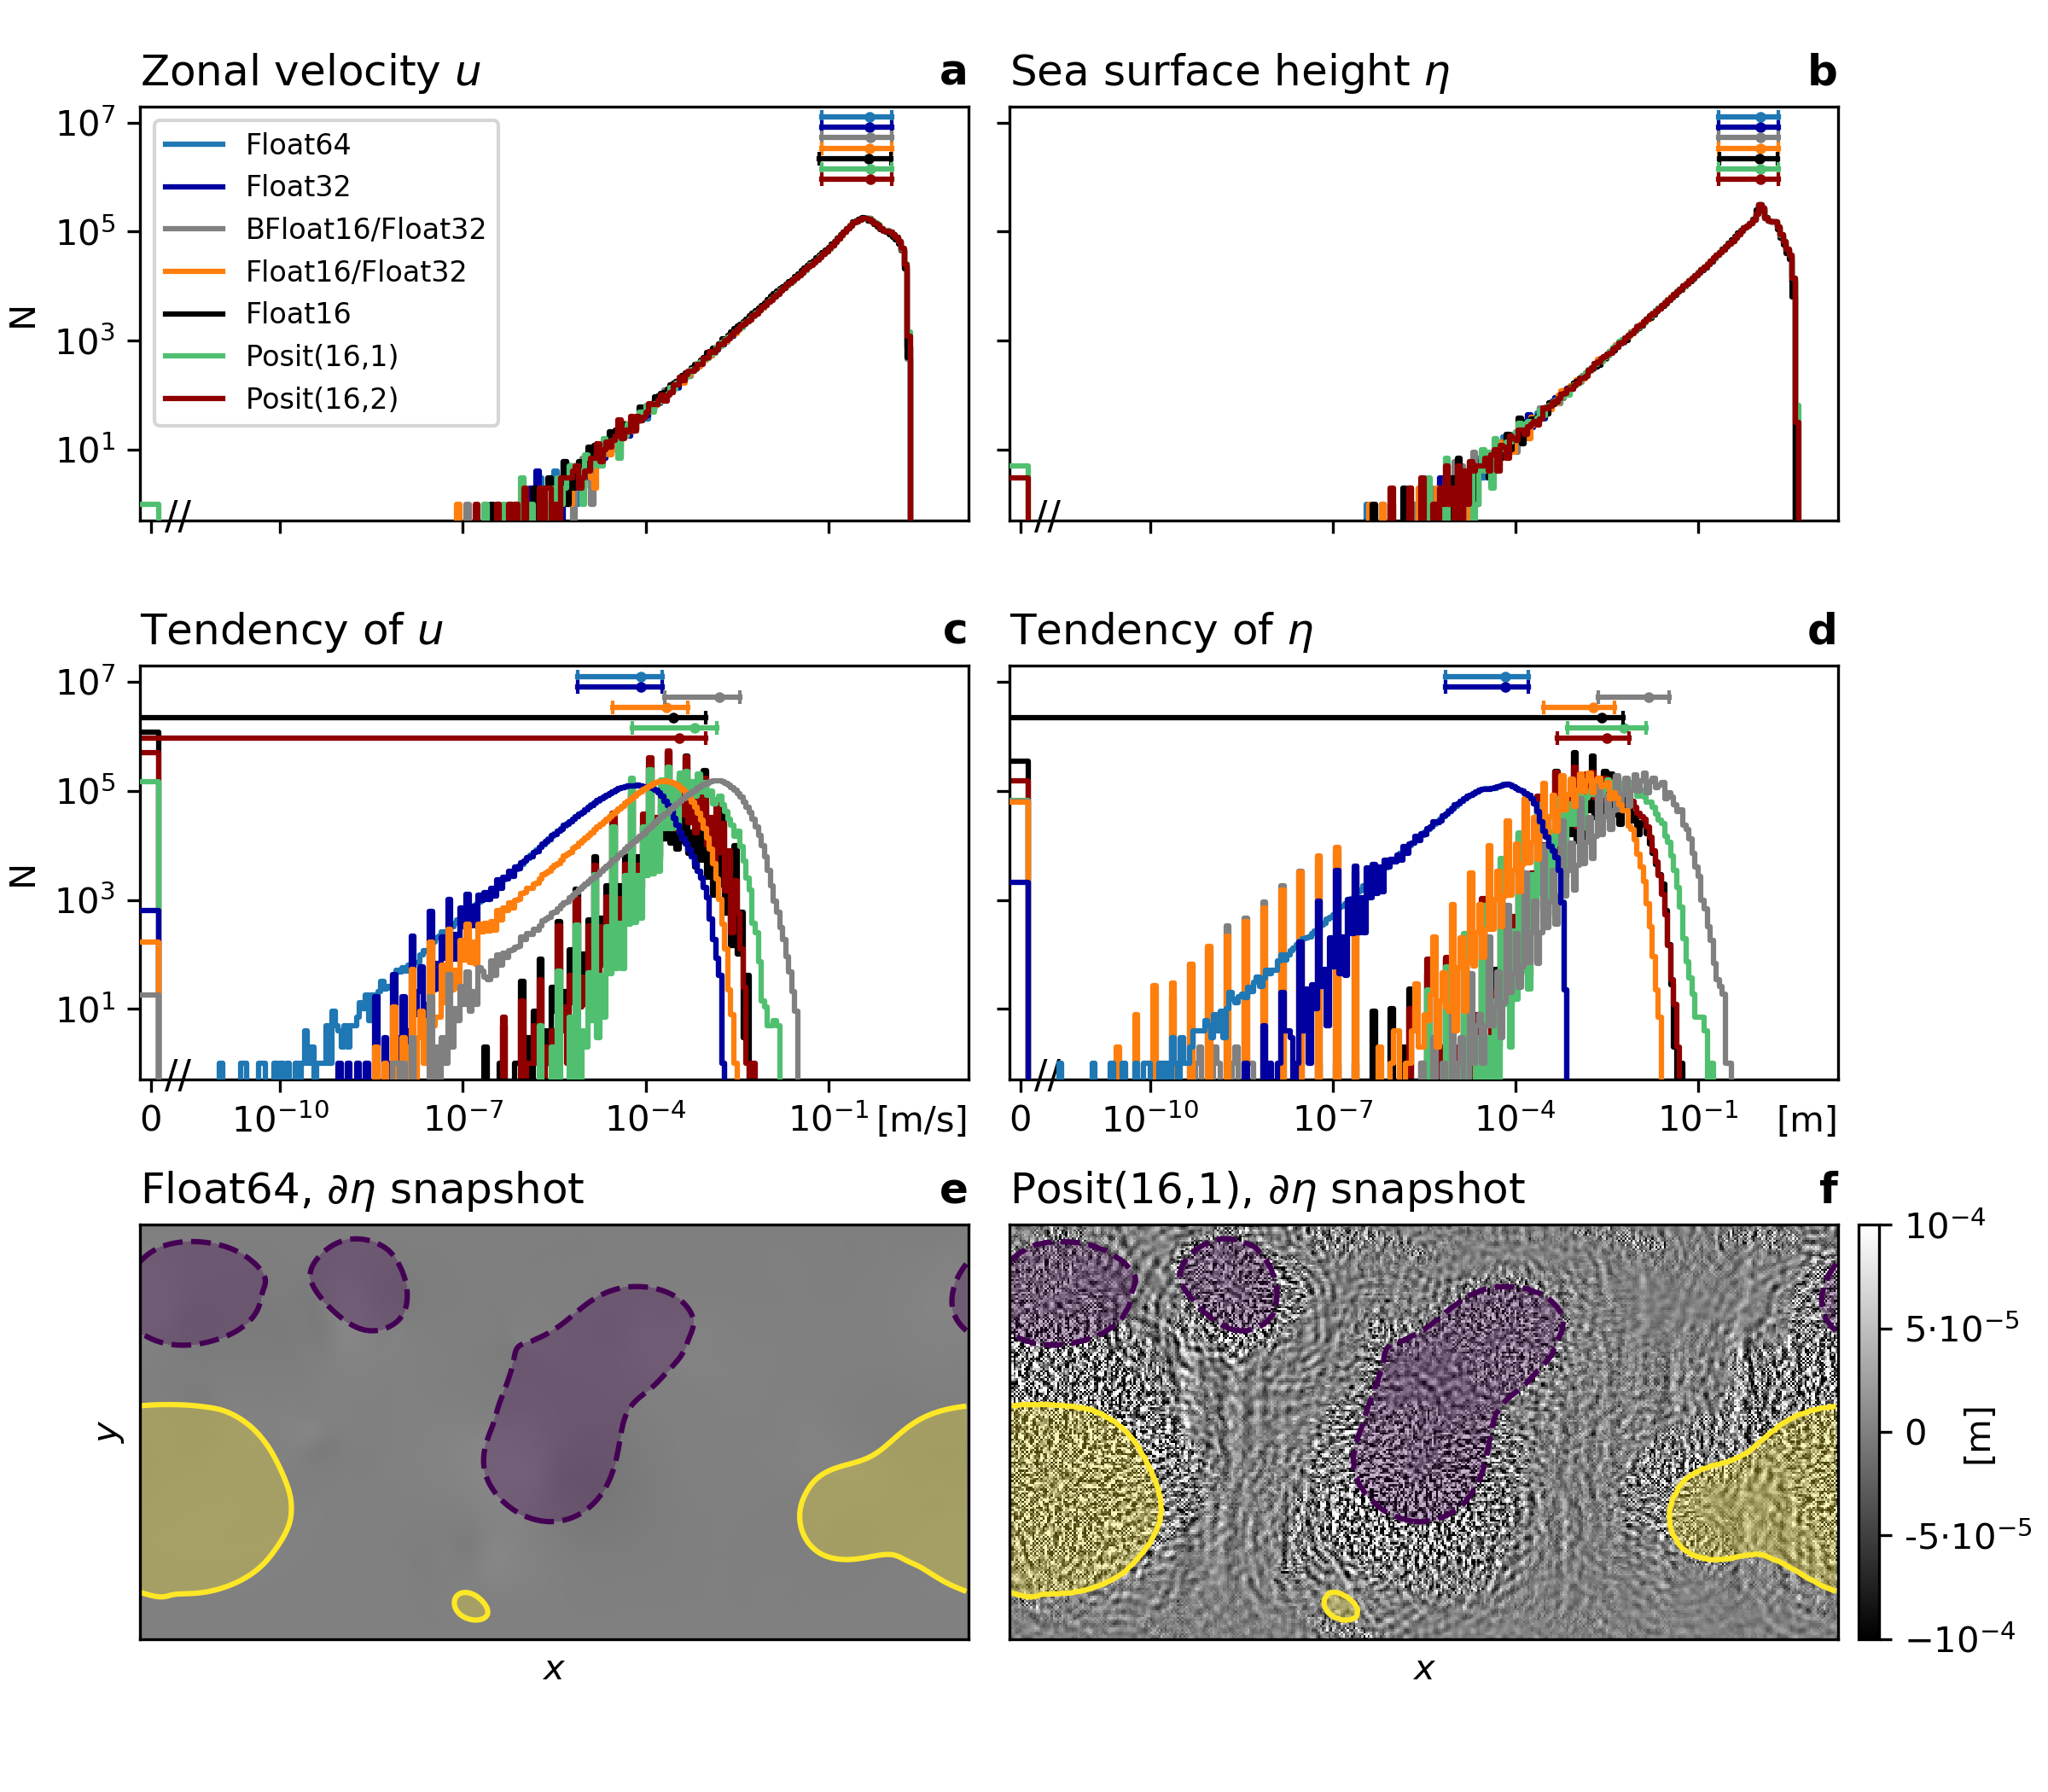
\includegraphics[width=1\textwidth]{tendency_hist.png}
\caption{Histograms of the numeric values of the prognostic variables (a) zonal
velocity $u$, (b) sea surface height $\eta$, and the respective tendencies of
(\change{d}{c}) $u$ and (\change{e}{d}) $\eta$, simulated with different 16, 32
and 64-bit number formats. Mean, 10th and 90th percentile are shown above the
histograms in respective colors. Snapshots of the tendencies of $\eta$ simulated
with (\change{c}{e}) Float64 and (f) Posit(16,1). Snapshots are similar for other 16-bit formats
(not shown here). Areas of sea surface height anomalies exceeding $\pm1.4$~m are
shown in purple (negativ\add{e}) and
yellow (positive). Note the break on the x-axis close to zero in (a,b,d) and (e).}
\label{fig:tend}
\end{figure}

As 16-bit arithmetics have no significant impact on the climatological mean state,
histograms of prognostic variables are also not changed (Fig. \ref{fig:tend}a and b).
However, the tendencies are increased by orders of magnitude with 16-bit arithmetics
(Fig. \ref{fig:tend}d and e), as rounding errors cause gravity waves to radiate
away from eddies (Fig. \ref{fig:tend}f). Gravity waves are identified from the
tendency of sea surface height. Comparing their propagation to the location of
anomalous sea surface height, which is used as a proxy to locate eddies, we
assume that rounding errors in regions of high eddy activity lead to instabilities
that propagate away in the form of gravity waves. These gravity waves are not
present in Float64 simulations (Fig. \ref{fig:tend}c) and tend to have only a
small impact on quasi-geostrophic dynamics, as they act on different time and
length scales. It is unclear but possible that gravity waves cause the observed
increased ageostrophic velocities for 16-bit arithmetic.

Tendencies are about 4 orders of magnitude smaller than the prognostic variables.
This poses a problem for number formats with a machine epsilon, measured as decimal
precision, significantly lower than 4 decimal places (Table \ref{tab:formats}).
Float16 has a machine epsilon of 3.7, which is presumably close to the lower limit
beyond which the addition of tendencies will be round back. The BFloat16 number
format has a machine epsilon of 2.8, which explains why flow is stalling when
simulated with BFloat16.

\subsection{Mixed precision arithmetic in the shallow water model}
\label{sec:mixed}

In the previous simulations the entire shallow water simulation was performed
with the specified number format. As the addition of tendencies to the prognostic
variables was identified as a key calculation that is error-prone, we investigate
now the benefits of mixed precision arithmetic, where Float32 is used for the
prognostic variables but the tendencies are computed with either Float16 or
BFloat16, two number formats that have the lowest decimal precision around 1.
The prognostic variables are now reduced to Float16 or BFloat16 before calculations
of the right-hand side and every term of the tendencies is converted back before
addition to the prognostic variables. Using subscripts 16 and 32 to denote variables
held at 16 and 32-bit precision, respectively, and let Float32() be the conversion
function. The continuity equation (Eq. \ref{eq:swe}b) then becomes
\begin{equation}
\frac{\partial \eta_{32}}{\partial t} = -\op{Float32}( \partial_x(u_{16}h_{16})
+ \partial_y(v_{16}h_{16} ))
\label{eq:conversion}
\end{equation}
and similar for $u$ and $v$ in Eq. \ref{eq:swe}a.

Snapshots of tracer concentration reveal well simulated geostrophic turbulence
(Fig. \ref{fig:snapshot}e and f) with Float16/Float32 or BFloat16/Float32 and
instabilities at fronts or in filaments are visibly reduced compared to pure
16-bit arithmetic. The forecast error is strongly reduced once the prognostic
variables are kept as Float32 (Fig. \ref{fig:rmse}a), supporting the hypothesis
that the addition of tendencies to the prognostic variables is a key computation
with low rounding error-tolerance. Despite BFloat16 not being suitable for shallow
water simulations when applied to all computations, mixing BFloat16 with Float32
arithmetic yields a similar error growth to posits, which is well below the
discretization error. Mean state or variability are virtually identical for both
mixed precision cases (Fig. \ref{fig:mean}) compared to the Float64 reference.
The geostrophic balance is largely unaffected, but ageostrophic velocities increase
in variance, especially for BFloat16 (Fig. \ref{fig:geo}). Gravity waves are
similarly present for mixed precision although weaker for tendencies computed
with Float16 (Fig. \ref{fig:tend}d) and, as discussed, they tend to not interact
with the geostrophic time and length scales. Although the results show that Float16
is generally a preferable number format over BFloat16 for the applications presented
here, we acknowledge that the conversion between Float32 and Float16 will come
with some computational cost. In contrast, the conversion between BFloat16 and
Float32 is computationally very cheap as both formats have the same number of
exponent bits. Removing significant bits, applying rounding, and padding
trailing zeros, are the only operations for this conversion. Following the
results here, mixing 16 and 32-bit precision is found to be an attractive solution
to circumvent spurious behaviour due to 16-bit floating-point arithmetics.
Performance benefits are still possible as most calculations are performed with
16 bit, with error-critical computations in 32 bit to reduce the overall error.

\add{Using mixed-precision in our shallow water model, 77\% of the arithmetic
operations are performed in 16 bit and the remaining 23\% in 32 bit. Assuming
Float16/BFloat16 to be two times faster than Float32 and conversion costs to
be negligible this would yield another 40\% reduction in computing time on top
of a reduction from Float64 to Float32. However, this depends on the soft
and hardware implementation considered. Some of the 16-bit accelerators (GPU/TPU)
can increase the flop rate by more than a factor of 2 when compared to Float32.
In addition, the shallow water model regarded here has a comparably simple
right-hand side, such that more complex models will spend more time to compute
tendencies which will come with a larger performance increase.}

\change{The conversions between number formats are likely of negligible cost. This}{
Mixed-precision} is an attractive solution as hardware-accelerated 16-bit
floating-point arithmetic is already available on graphic or tensor processing
units and implementations therefore do not rely on the development of future
computing hardware, which is the case for posits.

\begin{figure}
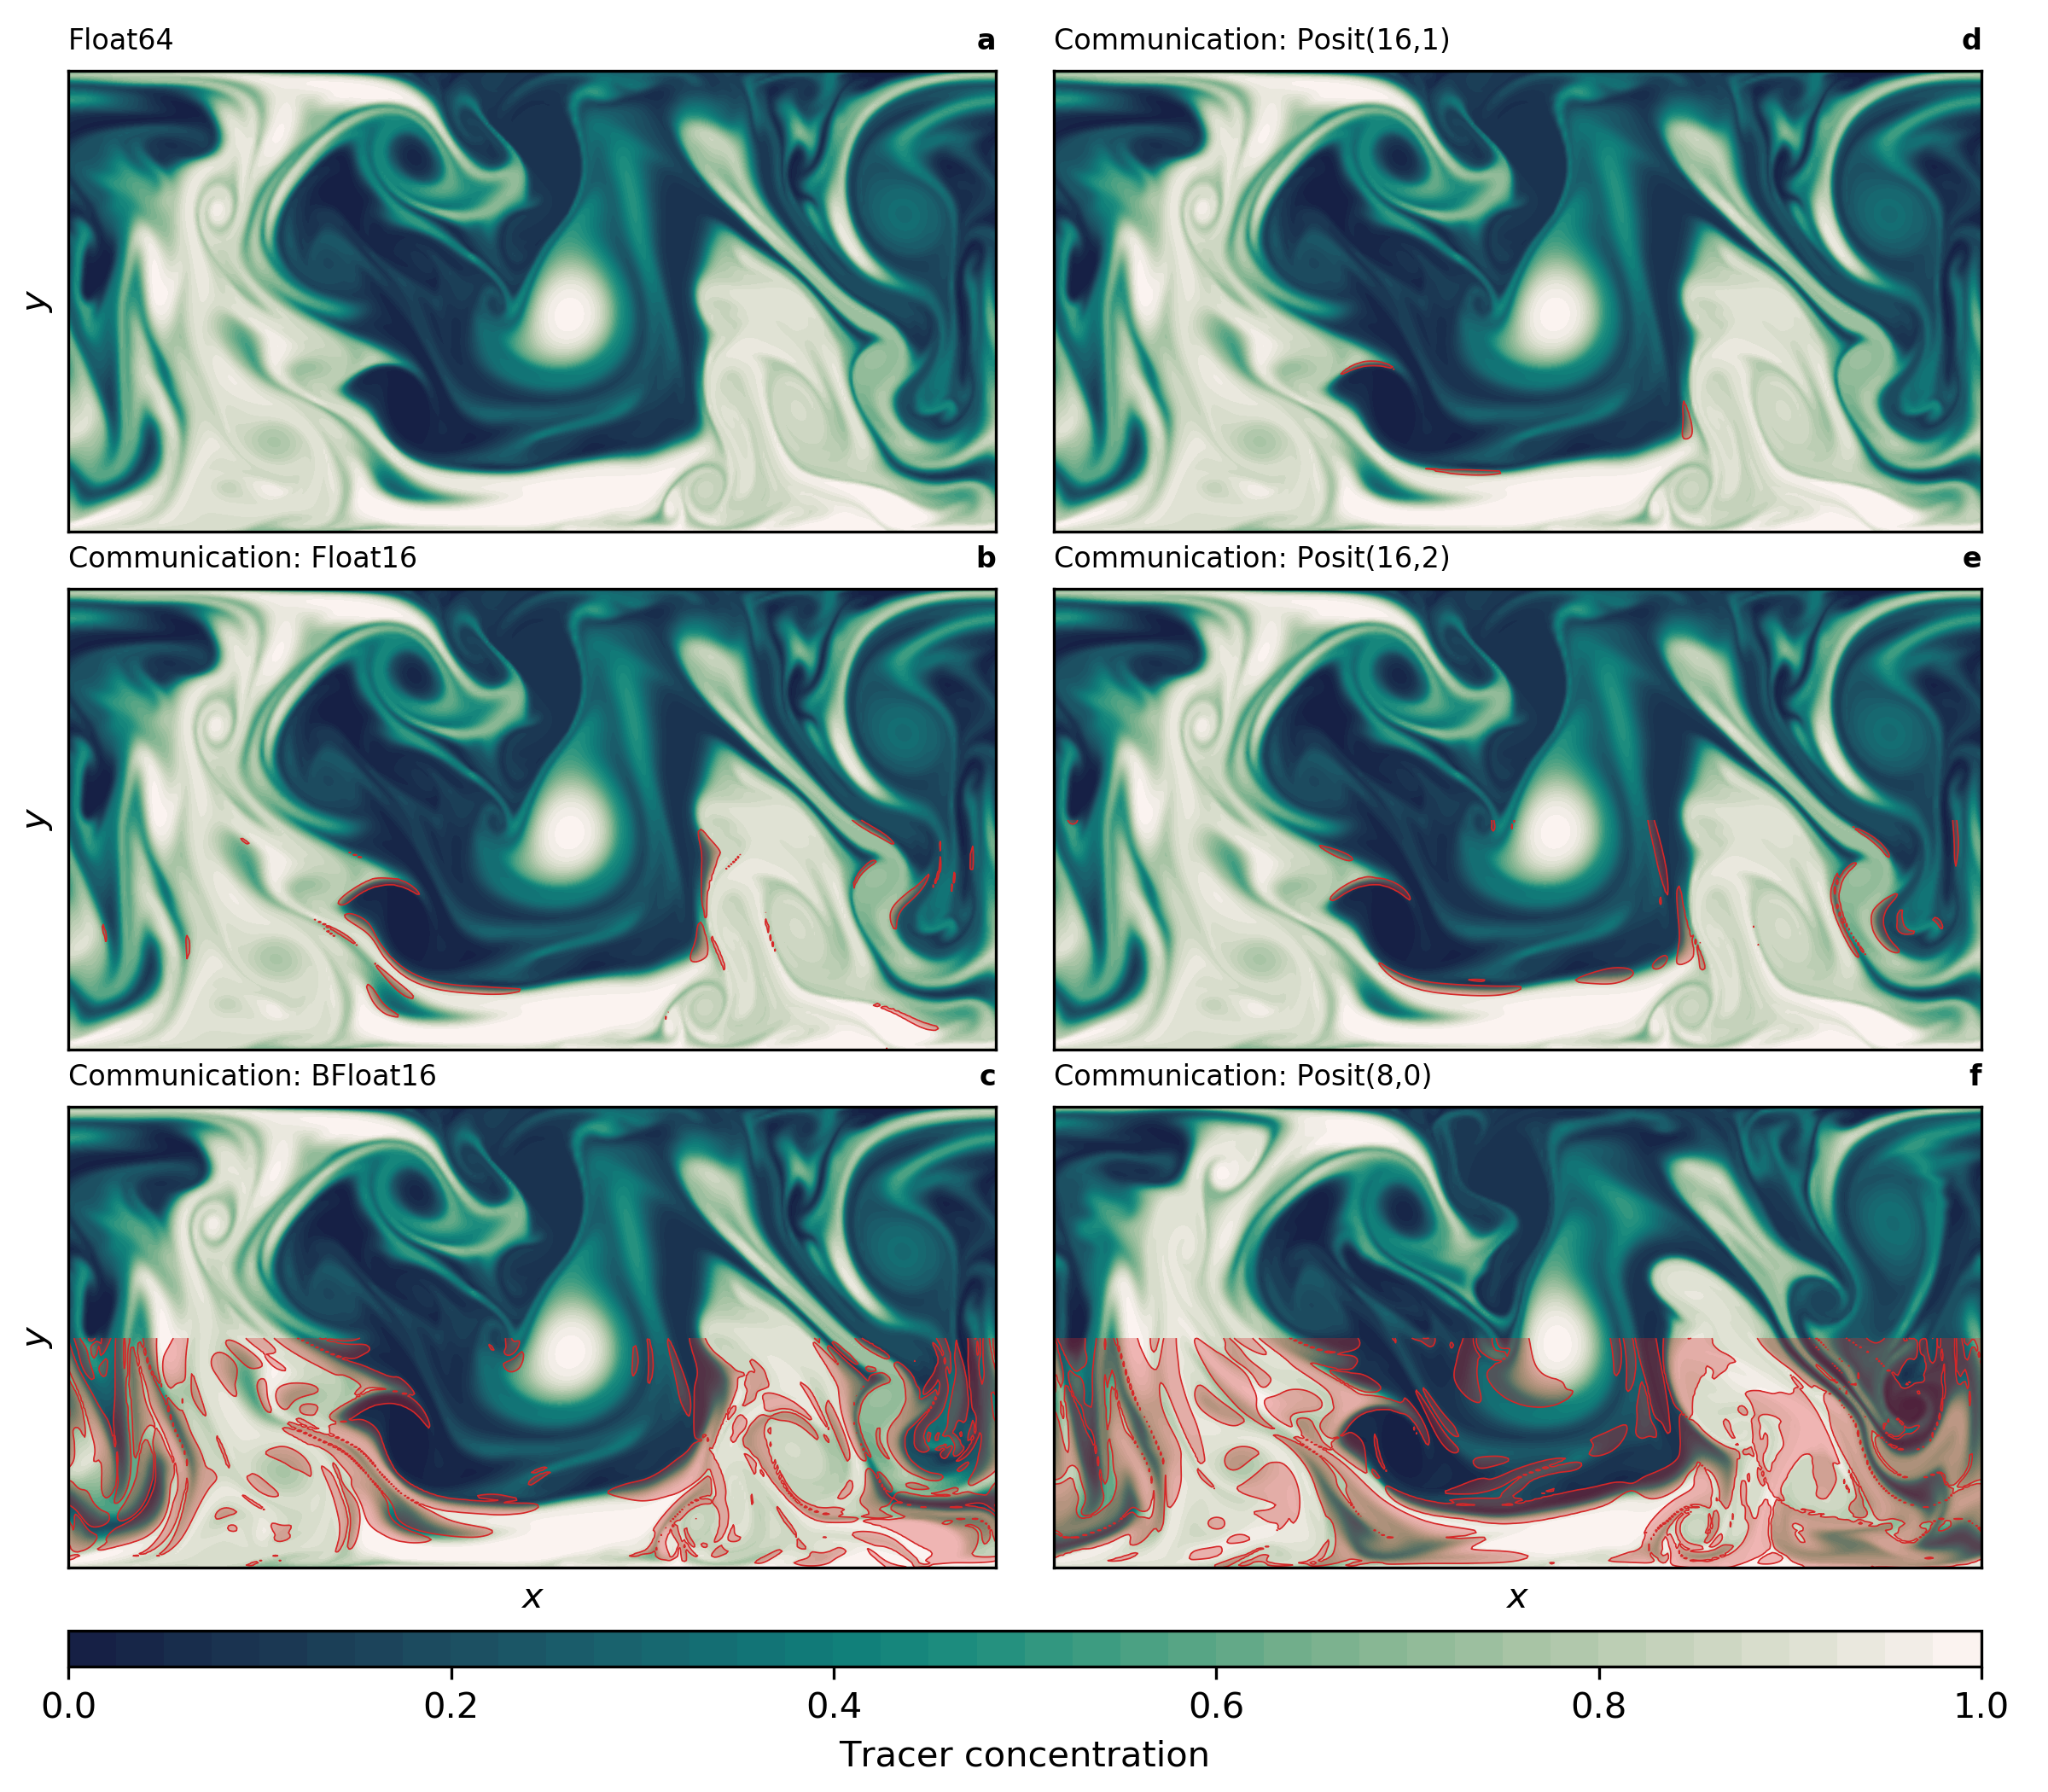
\includegraphics[width=1\textwidth]{snapshot_comm.png}
\caption{Snapshot of tracer concentration simulated by the shallow water model
using reduced precision communication. The communication of boundary values occurs
at every time step for the prognostic variables. Float64 was used for all calculations.
Areas where the absolute error exceeds 0.05 are shaded in red only in the lower
half of the domain. The tracer was injected uniformly in the lower half of the
domain 50 days before. This simulation was run in the high-resolution
configuration ($\Delta = 5$km).}
\label{fig:snapshot_comm}
\end{figure}


\subsection{Reduced precision communication for the shallow water model}
\label{sec:comm}

A standard method to parallelise simulations is the distributed-memory parallelism
via Message Passing Interface (MPI). We emulate MPI-like communication in the
shallow water model with the copying of boundary values between the right and
left boundary (periodic boundary conditions). Although the shallow water model
does not run in parallel, reducing the precision in the copying of boundary values
introduces an equivalent error as if reduced precision MPI communication was used
between subdomains. Reduced precision is applied for the communication of the
prognostic variables at every Runge-Kutta substep.

Regarding snapshots of tracer concentration simulated with reduced precision
communication shows a negligible error for Float16 and posits (Fig. \ref{fig:snapshot_comm}).
The error is largest at fronts and not concentrated around the boundaries.
Encoding the communication with BFloat16 introduces a larger error than for the
other 16-bit formats as the decimal precision is with 2.8 clearly lower
(Table \ref{tab:formats}) for the range of values occurring within the prognostic
variables (Fig. \ref{fig:tend}a and b). The errors are quantified by the RMSE of
surface height $\eta$ as before and are up to about two orders of magnitude smaller
than the errors that result from 16-bit arithmetic. As even the worst 16-bit
communication format, BFloat16, has a smaller error than the best mixed precision
formats, Float16 with Float32, we extend the short-term forecast experiments to
include two 8-bit formats, Posit(8,0) and Float8 (see Table \ref{tab:formats} for
a description). Both formats are found to be suitable for reduced precision
communication here and do not introduce an error that is larger than the
discretization error. Having said that, Float8 communication introduces an error
that is comparably large in the first days but growths only linearly in the first
50 days of the simulation, which is in contrast to the exponential error growth
observed for 16-bit arithmetic.

\section{Conclusion and Discussion}
\label{sec:discuss}

Future high performance computing architecture will support some 16-bit
arithmetics. The wall-clock time for weather and climate simulations could
be greatly reduced if computationally demanding algorithms were run at such
reduced precision. We tested a number of options for 16-bit arithmetic for
weather and climate applications in a shallow water model. The best results
were achieved with 16-bit posits (with either 1 or 2 exponent bits) which appear
very promising for application in high performance computing for Earth System
modelling. Float16 can be used to perform forecasts with the shallow water model
while the application of BFloat16 or integer arithmetic was not successful.

In general, 16-bit arithmetics were not found to alter the climatological mean
state or the large-scale dynamics. However, variability and ageostrophic velocities
were increased, such that second and higher-order statistics should undergo
testing to assess the models reliability. Depending on the application, an increased
variability does not necessarily deteriorate the model, especially for more
realistic model set-ups than considered here. However, our findings suggest that
reduced precision changes need to be done carefully as specific simulation features
can change without obvious impact on mean diagnostics.

Shallow water simulations with 16-bit arithmetic required rescaling of some terms
but no major revisions of the model code or algorithms. Given that only floats are
currently hardware-supported, we investigated mixed precision approaches.
Keeping the prognostic variables at 32 bit while computing the tendencies in 16 bit
reduced the rounding errors significantly. We also showed that numerical precision
for communication between compute nodes can be greatly reduced down to 16 or
even 8-bit without introducing a large error. Reduced precision communication was
not found to have a significant impact on either mean state, variability,
geostrophy or tendencies.

A \emph{perfect model} is used in this study, such that any form
of model or initial condition error is ignored and only the number format is
changed between simulations. Solely discretisation errors are estimated by
lowering the spatial resolution by a factor of 2. Although this is essential
here to analyse the impact of rounding errors isolated from other errors, it
is in general not a realistic configuration for weather or climate models. More
complex models include many other sources of forecast error, such that the
contribution of rounding errors from 16-bit arithmetic would likely be dwarfed by
model, discretisation or initial condition errors.

Only the most common discretisation method for fluid dynamics was used in
this study: Finite differences with an explicit time stepping scheme. But various
other discretisation methods exist, such as finite element or volume, spectral
methods and implicit time stepping. These methods come with different algorithms
and associated precision requirements. Consequently, some might be
less tolerant to rounding errors than the method used in this study.

\change{As there is no hardware available for posit arithmetic that we could have used
for performance testing, we cannot draw any conclusion about the performance of
posit arithmetic operations in comparison to Float16 or the other formats.}{There
is currently no hardware available for posit arithmetic that we could have used
for performance testing and it is seems impossible to make credible estimates
whether such hardware would be faster or slower when compared to hardware
optimised for Float16 arithmetic (as this does not only depend on theoretical
considerations but also on investments into chip design). We therefore cannot
draw any conclusion about the performance of posit arithmetic operations in
comparison to Float16 or the other formats.}

Until progress is made on hardware implementations for posits, the results here
suggest that also 16-bit float arithmetic can successfully be used for parts of
complex weather and climate models with the potential for acceleration on graphic
and tensor processing units. It is therefore recommended to adapt a type-flexible
programming paradigm, ideally in a language that supports portability, with
algorithms written to reduce the dynamic range of arithmetic results. Hardware
progress on central, graphic or tensor processing units, with various numbers
formats supported, can subsequently be utilised to accelerate weather and
climate simulations.

\acknowledgments
Milan Kl\"{o}wer and Tim N. Palmer gratefully acknowledge funding by the European
Research Council under grant number 741112 \emph{An Information Theoretic Approach
to Improving the Reliability of Weather and Climate Simulations}. Milan Kl\"{o}wer
is also funded by NERC grant number NE/L002612/1.  Peter D. D\"{u}ben gratefully
acknowledges funding from the Royal Society for his University Research Fellowship
as well as funding from the ESIWACE2 project. ESIWACE2 has received funding from
the European Union's Horizon 2020 research and innovation program under grant
agreement 823988.

Scripts and software is available at
\url{https://github.com/milankl/ClimateModels16bit}. Link will be converted to
DOI upon acceptance.

\bibliography{bibliography_new2}

\end{document}
